\chapter{Xenotech}

\begin{wrapfigure}{O}{\figwidth}
	\begin{center}
		
\includegraphics[width=\figwidth]{pics/11/1.png}
	\end{center}
\end{wrapfigure}
Junior Enginseer Jim had spent the last few days discussing the problem with Junior Enginseer Hannah. 
Neither of them had managed to think up any clever solutions and there was no one else to turn to. 
Asking the senior tech-priests for advice was right out, since they were half the problem anyway, and Ol' Bill just didn't understand the issue. 
In the end it was decided that their only option was to approach the problem directly. 
Which is to say Jim would approach the problem directly, Hannah refused to go anywhere near that section of the ship.

During his next nightly "Seventy Five Minute Organic Recuperation Period" Jim visited the storage room across from the Gellar Field Generator. 
Remembering it was Tuesday and after 1800, he bypassed the first two doors and made his way to the third where the mechanical keypad he'd expected had been replaced by a dataslate and a piece of yellow paper. 
Jim tried to ignore the claymore mine mounted underneath the slate as he read the note, it was labeled "Prove You Are Not a Servitor (or Ork)." A second smaller note said "cAsE sEnSiTiVe."

It took two tries to get the illegible series of hand-written letters entered into the slate, luckily the mine had only armed and the slate had instructed him not to move after the first mistake. 
Jim thought it was rather unfair to expect someone to be able to tell the difference between a lowercase and capital S. 
When the door finally opened the Enginseer made his way down a zig-zagging corridor of sandbags. 
As he walked he idly wondered where they'd managed to find sand on a voidship, then decided he was happier not knowing. 


When Jim came around the last bend he found three of the men he'd come to see piling up pieces of burnt meat and metal into a wheelbarrow. 
He ignored what looked like the remains of an unfortunate maintenance servitor and hesitantly asked if the Interrogator was present, or maybe even Doc.

\begin{wrapfigure}{O}{\figwidth}
	\begin{center}
		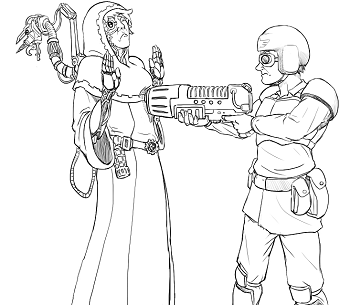
\includegraphics[width=\figwidth]{pics/11/2.png}
	\end{center}
\end{wrapfigure}
The shortest and most amiable of the three troopers, Nubby, explained that Sarge was working with the adepts and Doc was staying in the medbay on account of his legs not working. 
Several complex and undeniably obscene gestures accompanied this, either conveying Nubby's opinion of the adepts or what he thought Doc's actual reason for staying in the medbay was. 
Jim wasn't sure which.

Twitch interrupted the show to ask Jim if he was here about the servitor, because that was entirely not-Twitch's fault. 
He'd clearly explained that no-one was to attempt to clean or do maintenance on this room without an escort. 
Also, sharing access codes, even if it was with a servitor, was a severe violation of proper security protocol. 
Actually, change that to ESPECIALLY if it was with a servitor, those damned things couldn't be trusted; 
Jim should know, he'd been there and seen what the psychotic murder machines had done the second they got a chance.

Jim shuddered at the memories Twitch's rant dredged up, then turned to the third guardsman. 
While the other two had been talking Tink had been having a quiet, one-sided argument with the small xeno-tech dataslate he was holding. 
Occasionally he'd switch from swearing at the controller to cooing at the hovering disk in front of him as it tried, with mixed success, to pick up pieces of servitor with its small servo-arm. 
Jim summoned every scrap of courage he could muster and walked up to the goggle-wearing guardsman. 


"Tink, this tech-heresy needs to stop. 
If you don't destroy that unholy xenos contraption I will-I will-I, um, uhhhh, pleasedon'tkillme." 

Tink pressed the the humming plasma gun, which Jim swore he hadn't been holding second ago, a little harder into the enginseer's chest. 
In the most threatening voice he could muster, Tink asked:

"What did you just call my waifu?"

\greentext{>The All Guardsmen Party and the Xeno-Tech Heresy}


\begin{wrapfigure}{O}{\figwidth}
	\begin{center}
		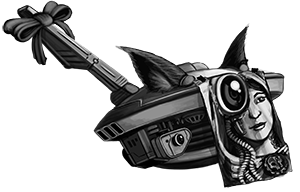
\includegraphics[width=\figwidth]{pics/11/3.png}
	\end{center}
\end{wrapfigure}
Nubby came to Jim's rescue before long. 
He carefully pushed the plasma gun to the side and reminded Tink that Sarge had banned the "W Word". 
Furthermore, this was Jim, the bro-est of cogbros! 
He was definitely on the do-not-blow-in-half with a plasma gun list, and hadn't meant to insult Tink's favorite toy. 
There was undoubtedly a reason behind his request and if everyone would just settle down this could all be sorted out without Sarge yelling at anyone.

Tink grumbled about it not being a toy. 
SHE was a DX-9F Exploratory Drone, configured for stealth operations and tech interfacing, and HER name was "Hannah Two-Point-Oh". 
Jim went blank as he processed this, then started sputtering in a mix of shock and revulsion. 
Nubby groaned and waved a hand at Twitch, who obliged by pegging the ranting trooper in the back of the head with a chunk of servitor. 
Both parties were hauled off and seated in front of one of the several whiteboards that had gone missing from the official briefing rooms. 


Jim boggled at the list on the board as the Nubby forced a surly Tink to read off the last six items on it.

SARGE'S XENO-TECH RULES
\greentext{>1. Keep your stupid mouths shut.}

\greentext{>2. If you want to use a weapon it MUST be disguised as a lasgun or something. THIS INCLUDES YOUR PLASMA HYBRID MONSTROSITY.}

\greentext{>3. The drone is SECRET. It does not leave the barracks unless it's in its box or you can make it look like a servo-skull.}

\greentext{>4. Sarge will be the judge of whether the drone ACTUALLY looks like a servo-skull.}

\greentext{>5. The drone is NOT a she.}

\greentext{>6. The drone does NOT have a gender at all.}

\greentext{>7. The drone is NOT named Hannah or Fio'whatsit.}

\greentext{>8. The drone is NOT named after ANYONE, regardless of if we've met them.}

\greentext{>9. The drone is named Spot. It is a good name and is actually sort of witty. All complaints must be hand-written and submitted in person to Interrogator Sarge.}

\greentext{>10. Anyone who violates these rules or actually submits a complaint will be made to suffer in ways they cannot possibly imagine.}


\begin{wrapfigure}{O}{\figwidth}
	\begin{center}
		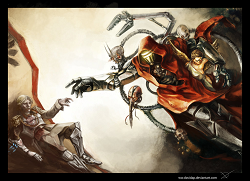
\includegraphics[width=\figwidth]{pics/11/4.png}
	\end{center}
\end{wrapfigure}
After the base rules were re-established and Tink had accepted that no-one was going to be allowed to shoot anyone, unless it was Twitch and there was an Ork attack, Nubby asked Jim what the problem was. 
If he was here about our recent acquisitions, it should be obvious that we had the situation in hand. 
Everyone was aware of the Mechanicus' little rules about xeno-tech and would be keeping a low profile, so no worries. 
None of us were ready for the explosion that the phrase "little rules" triggered. 


The young enginseer leapt out of his seat and started pacing back and forth, frantically explaining that this wasn't a matter of laws or protocol, this was dogma. 
See cogboys tend to be a little more religious when it comes to technology than most guardsmen. 
Which isn't surprising, they're called TECH-PRIESTS after all, but the exact nature of their religion is a little complex. 


Some of them loved all tech, especially the old and complex stuff, and would go around worshiping random things they dug out of space hulks. 
Others were all for getting and keeping their technology working as well as possible or maybe even pulling apart things to see how they work. 
Some cogboys though, were completely focused on stamping out any piece of tech, no matter how amazing, that didn't originate from Mars. 
According to Jim, about half the senior tech-priests on the ship fell into that last category.

\begin{wrapfigure}{O}{\figwidth}
	\begin{center}
		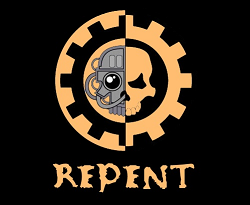
\includegraphics[width=\figwidth]{pics/11/5.png}
	\end{center}
\end{wrapfigure}
Jim claimed these were the sort of guys who wouldn't just destroy a device they suspected of being xenos-made, they'd also convert anyone who'd ever used it into servitors, then push the servitors into a plasma reactor. 
Nubby suggested that this was a bit of an exaggeration, the Inquisition always got a fair bit of leniency on this stuff. 


Didn't that Interrogator with the big hat have a sword that whispered at anyone nearby about drinking their blood? 
What about sister what's-her-face who had a Sternguard Pattern Bolter that she'd looted from a dead marine? 
And no one commented on the fact that the guy running recruitment had actually purchased a medium-sized tropical island with the funds he'd been embezzling over the last few decades. 
Surely a little xeno-tech could be swept under the same rug those guys were using. 
Jim just shook his head and pointed out that all those were things that the Inquisition typically had jurisdiction over; 
believe it or not, hardcore orthodox tech-priests were a lot less forgiving.

Jim suggested that as a baseline we imagine a three hundred year old Redemptionist preacher. 
Now combine that general cranky outlook with the fact that the orthodox tech-priests on the ship had been forced to accept that most of its critical engineering staff were not members of the machine cult. 
These guys were itching to put someone in their place; 
if ayone caught their attention with a clear case of tech-heresy, their lifespan would be measured in minutes. 
So Jim was asking, begging really, for us to give up or suicidal fascination with xeno-tech.

\begin{wrapfigure}{O}{\figwidth}
	\begin{center}
		
\includegraphics[width=\figwidth]{pics/11/6.png}
	\end{center}
\end{wrapfigure}
Everyone went quiet for a while as they processed this. 
Tink frowned at his drone controller, Twitch pondered how many servitors those priests commanded, and Nubby weighed the value of his life against that of a crate of Tau pulse weapons. 
All of us looked at each other and came to a silent agreement. 
Nubby thanked Jim for his warning, it'd really opened our eyes to the situation. 
He promised that we would… be very careful not to show their new toys to any tech-priests. 
Except for Jim. 
And Hannah. 
Oh and those other guys we couldn't remember the names of, but had been pretty cool for cogboys. 


Jim sank into his seat and looked like he was about to start crying. 


While Twitch and Tink went back to cleaning, Nubby did his best to console the young enginseer. 
Eventually his weasley arguments about how unlikely the senior tech-priests were to find out, if no one ratted to them that is, calmed Jim down. 
From there it wasn't hard to convince him to help with the "disguise the xeno-tech" project. 
Given how much damage a minor war located across the hall from the Gellar Field Generator would cause, Nubby argued, it could even be budgeted under preventive ship maintenance. 


The enginseer grudgingly sat down at the workbench Tink had been using for the project and started tinkering. 
He didn't even pause to question the origins of the pile of slightly-used lasguns or the large crate of assorted human and animal skulls that had been provided for camouflage material. 
He'd made some real progress and was even managing a nearly-civil technical discussion with Tink when Sarge came back.

Sarge, who'd spent at least twenty hours over the last few days trying to fill the gaps in his team left by Doc's injury and the Infiltrator's death, took Jim's presence as a sign from the Emperor. 
Before the night was over, the paperwork was in order and the enginseer was officially seconded to us for the duration of the upcoming mission.

Jim was not exactly happy about this.

\begin{wrapfigure}{O}{\figwidth}
	\begin{center}
		
\includegraphics[width=\figwidth]{pics/11/7.png}
	\end{center}
\end{wrapfigure}
That upcoming mission was a bit of a mystery. 
Our little op on the Tau border worlds had gone relatively well: 
We'd foiled a rather convoluted plot to get neutral worlds in bed with the Tau empire and killed the raiders that'd been terrorizing the area. 
At least we'd thought that the Rogue Trader we'd doomed to an incredibly gruesome death was behind all the missing colonies and stations, turned out his band of pirates didn't quite fit the bill though. 


It's not like they hadn't had it coming, no one but Doc felt guilty about trapping those mercenary bastards in the warp with no Gellar Field, but according to our reports whoever was wiping out the locals didn't leave bodies. 
Not theirs, and not their victims either. 
That was pretty ominous, especially coupled with the fact that a few of the other Inquisitorial teams on our little expedition had been on those worlds. 
None of them had sent out any messages, they'd just vanished with the civies. 
Yeah, ominous.

All those guys had been the same as us: 
small teams of underfunded, underinformed, and under-everything-else Inquisitorial agents sent out to look for trouble or do something for Oak. 
We were definitely the last people to suggest that they should have been able to stop some sort of colony-eradicating doom-thingy… But we'd have expected them to at least get SOMETHING out. 
Even if it was just an astropath message saying "Shit. 
Tyranids." or "I FEEL THE WARP OVERTAKING ME. 
IT IS A GOOD PAIN." They didn't though, which meant that whatever had gotten them was even weirder than usual.

All we had to go on was the information the Occurrence Border's captain had scrounged for us when the teams had missed their pickups. 
He had a rough map of which systems had been wiped out for sure and a few notes from the one colony he'd personally inspected. 
That's how we knew he was worried, the Captain didn't like going down to planets. 
He said they were untidy.

\begin{wrapfigure}{O}{\figwidth}
	\begin{center}
		
\includegraphics[width=\figwidth]{pics/11/8.png}
	\end{center}
\end{wrapfigure}
The disappearances charted a sort of winding path through the region, starting on the fringe of Tau space and twisting in the general direction of the Imperium. 
That was the whole reason we were involved in this mess. 
None of us gave a shit if a bunch of xenos got killed or really cared much about the fringe worlds, but if the pattern continued some valuable Imperial worlds were going to get wiped out. 
So Oak had mandated that everyone out here was to drop what they were doing and figure out what the hell was going on. 
The Occurrence Border had picked up all the teams it could reach in time and was doing its best to follow the trail before it got cold.

Sarge spent a lot of time working with the adepts and the other teams to figure out what we were in for before we ran right into it. 
Sarge had sat down with the Captain, who he got along with rather better than the other Interrogators and gone over the whole thing from top to bottom. 
Unfortunately, all they were able to figure out was that the path mostly followed decent warp routes, which told us whoever was driving was probably using a Warp-Drive. 
Or they just felt like going that way.

The Captain's brief visit to the purged colony had turned up some more useful info. 
He'd described the place as being mostly intact, but with no creatures, living or dead. 
There was some battle damage, but the place hadn't just been nuked from orbit and he said it didn't look like the fight had lasted long. 
Sarge tried to pick his brain for details about the battle damage, hoping to pin down what sort of weaponry had been used, the Captain wasn't much help though. 
All he was able to tell us was that no one had used Macro Cannons, Lances, Torpedos, or Nova Cannons. 
Oh, and someone had dropped several million tonnes of powdered silicate and organic matter on the place, that struck him as interesting. 
A few probing questions revealed that this mysterious substance was, in fact, just the ground. 
Bloody spacers.

\begin{wrapfigure}{O}{\figwidth}
	\begin{center}
		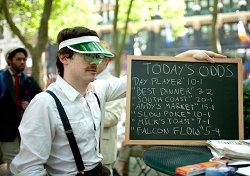
\includegraphics[width=\figwidth]{pics/11/9.png}
	\end{center}
\end{wrapfigure}
It was eventually decided that the only way we'd get anything useful was by visiting one of these worlds and looking around ourselves, preferably after the mysterious people-disappearing thing had left. 
Until then all anyone could do was wildly speculate, so we did what any red-blooded guardsmen would do in that situation: 
we started a betting pool.

At first it was the usual small wagers between us, everyone sticking to their pet theories and so on, but Nubby smelled profit and the thing quickly grew to ludicrous size. 
Within a few days both the other teams, the entire engineering department, and half of the ship's officers were in on it. 
There'd even been a runner from the Navigator's sanctum carrying bets from him and the Astropath, neither of whom had even been told about the pool. 
That'd sparked a lengthy debate about whether those guys could see the future and if that should invalidate their bets. 
In the end Nubby held that if they could, then they'd have been able to avoid being assigned to the Occurrence Border, so he took their money like everyone else's.

There wound up being only three popular bets since various factors wound up disqualifying most of the candidates. 
No one was willing to put money on it being some human force, on account of how Oak would've known if there was a rogue Inquisition fleet out here, and Chaos warbands or cults were never this tidy. 
On the xenos side the Tau didn't fit, Necrons tended to stick to their tomb worlds, Tyranids either left planets barren or full of Tyranids, and even Twitch couldn't figure out how it could be Orks. 
That just left warpy stuff, Eldar, or some really obscure type of xenos.

\begin{wrapfigure}{O}{\figwidth}
	\begin{center}
		
\includegraphics[width=\figwidth]{pics/11/10.png}
	\end{center}
\end{wrapfigure}
Sarge and Doc had their money on some sort of crazy warp shit, either a greater Daemon or some sort of massive phenomena. 
They didn't have any real reason behind the theory, but since it was the scariest thing anyone could think of it had a lock on the pessimist vote. 
Outside of the pool, all the adepts who knew about that warpy stuff were going through their records trying to figure out what could be done if they were right.

Meanwhile, after Twitch gave up on the Orks he'd gone down to the adepts and gotten a list of all the types of xenos that lived out on the fringe. 
He didn't sleep for three days after that and eventually had to be tranqued by Doc. 
Well by his girlfriend, Doc wasn't in any condition to chase down Twitch on account of the whole wheelchair thing. 
Anyway, after he was pried out of his hole, Twitch made a fairly strong case for some obscure xenos horrors being behind everything. 
Even Tink and our team's adepts threw in with him, either because they believed him or just thought it was good odds to play the field.

The final popular bet was the OCD Eldar Raiders theory. 
Nubby and Fumbles had started that one by hotly denying that it was even a possibility. 
The denial had come right after they'd received the Navigator's bet, and even if most folks couldn't figure out why the Eldar would be disappearing colonies, they knew what a rigged game looked like. 
Nubby hadn't gotten any sympathy from the rest of us when he'd complained about how even the odds were getting.

\begin{wrapfigure}{O}{\figwidth}
	\begin{center}
		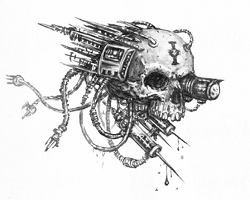
\includegraphics[width=\figwidth]{pics/11/11.png}
	\end{center}
\end{wrapfigure}
Between the pool, Tink and Jim's project, and Sarge's scramble to prep for the mission, Doc was the only one with much free time. 
Of course that was primarily because he was stuck in a wheelchair until his leg and gut-wound finished healing. 
He spent most of that time in the medbay acting as a handi-capable nurse for his girlfriend, and despite Nubby's constant barrage of tasteless jokes, seemed to be coping with his temporary crippling fairly well. 
We mostly left him to it, since we risked death by either sap overdose or angry hospitaller every time we visited. 
Twitch nearly lost an ear to a thrown scalpel when we kidnapped the poor boy for a night of recreational drinking.

While Doc wasn't too bothered about his injury, it was a constant source of worry for the rest of us. 
Not because we thought he wouldn't get better, but because the Captain had spotted a world in the right direction that had gone dark and was taking us there for a little reconnoitering. 
Our ETA was a few days, and Doc's recovery was going to be a matter of weeks or months, so it was looking like we'd be going into the field without a medic. 
Sarge and Jim tried to convince us that the medi-skull they'd requisitioned was just as good, but we weren't buying it. 
Those things are unsettling just to look at, they're a million times worse when you've just been shot and one's coming at you with a buzzsaw.

Everyone was feeling a little nervous when we finally came out of the warp and confirmed that the nearby planet was emptier than a Munitorum agent's heart. 
Those of us who weren't creeped out by the prospect of nosing around on a freshly depopulated world were wondering if we were about to lose three weeks pay in the pool. 


\begin{wrapfigure}{O}{\figwidth}
	\begin{center}
		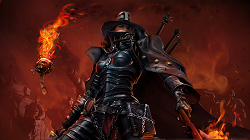
\includegraphics[width=\figwidth]{pics/11/12.png}
	\end{center}
\end{wrapfigure}
While everyone worried and prepped their gear Sarge attended one final meeting with the Captain and the other two Interrogators. 
Now these guys weren't bad sorts, at least by officer standards, but neither of them really played well with others. 
One was a blond battleaxe of an ex-cleric and the other was a serious agent fellow with a creepy sword that no one commented on. 


Battleaxe had been drumming up recruits and Sword-guy had been trouble-stabbing some problem for Oak before the new orders came through, neither of them was very happy about being reassigned mid mission. 
Despite their unhappiness they'd treated Sarge well enough and their adepts had worked with ours on the data processing, but no one was willing to accept anyone but themselves as the missions leader. 
That included Sarge, who'd immediately recognized two people who wouldn't blink at sacrificing a few guardsmen.

Since no one was feeling overly cooperative, the basic plan was for each team to send a separate party to the dead planet and look for clues. 
If anyone found anything interesting they'd call for the adepts, and if they found hostiles they'd call for reinforcements from the ship or the other teams. 
It wasn't the most efficient plan, but without some clear and present danger it was the best we were going to get. 
The final meeting between the three interrogators and the Captain was to determine who would go where on the planet and how much support the Occurrence Border would provide.

\begin{wrapfigure}{O}{\figwidth}
	\begin{center}
		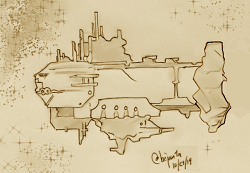
\includegraphics[width=\figwidth]{pics/11/13.png}
	\end{center}
\end{wrapfigure}
The planet was sort of shitty and probably had a population of only five or six million before it got wiped out. 
Battleaxe called dibs on what passed for the local center of government and Sword-guy wanted to take his team to the largest commercial shuttleport. 
Sarge carefully considered the remaining options, then ignored the pointed suggestions that he inspect the planet's only military base in favor of the smallest shuttleport on the planet. 
Sarge carefully deflected their questions about his choice with vague comments about hunches and feelings, he managed to hold out until the Captain got annoyed and forced the discussion move along.

It was agreed that the Occurrence Border would hang in stationary orbit and handle communications while each team was given their own shuttle. 
The emergency support options consisted of the remaining two shuttles loaded with all the armsmen the Captain thought he could reasonably spare and the ship's lances. 
Everyone was reminded that the last time those lances were used at that range they'd missed by seventeen kilometers and had to be walked, while still firing at full power and jiggling a lot, to their target. 
The Captain recommended not asking for any precision strikes then called an end to the meeting.

Sarge gathered us up in the shuttlebay for a final briefing before we went down. 
The ground team consisted of everyone except the adepts, who would be hanging out in the Comm room and analyzing whatever we sent to them, and Doc who was only in there to wish us luck before he went to get the medbay ready for whoever got shot this time. 
Hannah and Ol' Bill were there too, mostly to remind us that Jim was considered essential to the smooth-ish running of the ship. 
It would go poorly for us if he came back in anything less than factory-fresh condition.

\begin{wrapfigure}{O}{\figwidth}
	\begin{center}
		
\includegraphics[width=\figwidth]{pics/11/14.png}
	\end{center}
\end{wrapfigure}
Our briefing started with Sarge acknowledging that randomly walking around a deserted planet "looking for clues" was about the stupidest way of gathering information invented. 
This stole Tink and Nubby's thunder and shut them up for long enough for Sarge to explain our real mission, which was to hang out within support range of the other two teams. 
If something was going to try and kill nosy people, it'd probably start with them and we'd be in a good position to swoop in and save the day or make a clean escape. 
All we had to do was stay near the shuttle and keep out of trouble while the people who actually knew what a clue looked like did the hard work. 
It was a very good plan.

The cherry on top was the location Sarge'd picked for us. 
He'd chosen it for three reasons, firstly he'd figured that running around a military facility that was probably filled with partially activated defences and undetonated ordinance was incredibly stupid and no other locations really had anything tailored to our skills. 
Secondly it was pretty much between the other teams, which would make supporting them easier. 
Finally, the planet's climate was cold and wet and that tropical island shuttleport was the only credible location that wasn't currently being rained, snowed, or sleeted on. 
So yeah, we were going there because it looked like it would be a pleasant day at the beach. 
Doc and his girlfriend looked vaguely jealous as we boarded the shuttle.

We'd been offered a pilot for our shuttle, but two of us were qualified to fly the thing and we preferred having someone we really trusted in charge of our only transport. 
Also, Nubby pointed out that they might rat us out to the other teams. 
Tink and Jim had brief, heated debate about who was pilot and co-pilot, which ended poorly for both of them when their slap-fight over the joystick knocked over Sarge's recaff.

\begin{wrapfigure}{O}{\figwidth}
	\begin{center}
		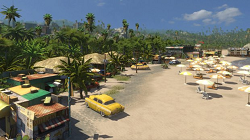
\includegraphics[width=\figwidth]{pics/11/15.png}
	\end{center}
\end{wrapfigure}
Aside from the brief excitement provided by Sarge chewing out the techies, the ride down was fairly boring, even the view out the window was dull. 
The top half of the planet was white with snow, the bottom half was mostly water or clouds, and even Nubby couldn't find any obscene looking continents. 
Twitch tried to liven things up by speculating on what type of xenos horrors had abducted everyone and what unspeakable things were being done to them, but stopped when Fumbles looked like he was going to start crying.

Our first look at the shuttleport confirmed Sarge's genius: 
the place was obviously built as some sort of vacation resort for rich merchants. 
A quick flyover turned up a complete lack of people, vehicles, or xenos monstrosities and an environment scan revealed nothing more dangerous than a chance of sunburn, so we set down right on there on the beach. 
There was a final comm check and reiteration of the ground rules, then everyone went off to enjoy themselves.

Now, you may be getting the impression that we weren't taking our mission as seriously as it warranted, and anyone from the other teams would've certainly said so. 
There's a difference between not being serious and not being effective though, and we fully intended to complete the objectives we'd set for ourselves. 


Since in our eyes our main job was to be ready to save the other teams' bacon, everyone stayed within sprinting distance of the shuttle and Jim kept its engines warmed up. 
In deference to the fact that this was potentially hostile territory everyone outside the shuttle stuck in groups and Twitch worked with Jim to set up a rudimentary perimeter around the LZ. 
Finally, Spot the wonder-drone was feeding everything it saw to our adepts and we were definitely keeping our eyes open as we strolled around the beach and inspected all the bungalows. 
Admittedly Nubby was the one doing most of the inspecting, but it's not like anyone expected us to find anything anyway.

\begin{wrapfigure}{O}{\figwidth}
	\begin{center}
		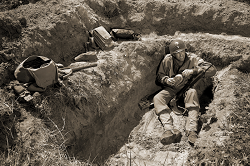
\includegraphics[width=\figwidth]{pics/11/16.png}
	\end{center}
\end{wrapfigure}
Sarge picked through a few beach-chairs until he found one that didn't have a big vaguely human-shaped hole in it, and made himself comfortable. 
He lounged in the sun and listened to the other teams' comm traffic, from the sound of it Battleaxe had already spotted the silhouettes and didn't to be pointed towards them. 
The burly noncom laid back and idly watched as Twitch built some truly impressive sand castles.

Jim elected to stay on the shuttle, claiming that sand was bad for his metal bits, but sent out a few servo-skulls and chatted with Tink over the comm. 
The techie had yanked off the two grox skulls his drone had been encased in, and was nauseating the adepts trying to watch the vid-feed by racing it against Jim's skulls. 
When they started arguing over whether ramming was allowed and if busting through walls should count as a penalty Sarge made them switch to hide-and-seek.

While everyone else stayed near the shuttle, Nubby grabbed Fumbles and went to do an exhaustive search of the nearby buildings. 
At first it was for small and valuable items that might need a new home, but after a while Nubby realized that he was being unprofessional. 
A few minutes later he and Fumbles had acquired a wheelbarrow and switched to searching for large and valuable items that might need a new home. 
Fumbles happily pushed the barrow and learned several important lessons about the difference between looting and recycling.

Everything was going splendidly and Sarge was considering taking a nap when Twitch screamed "MOVEMENT" and dove into a freshly dug sand-trench.

\begin{wrapfigure}{O}{\figwidth}
	\begin{center}
		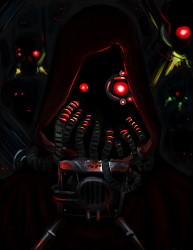
\includegraphics[width=\figwidth]{pics/11/17.png}
	\end{center}
\end{wrapfigure}
Despite the amount of shit the rest of us gave Twitch over his paranoia, we all trusted his spotting skills with our lives. 
Within seconds Sarge and Tink landed in the trench next to him and overhead the drone engaged its stealth field. 
On the far side of the shuttle Nubby and Fumbles dropped their loot and got ready to either flank or sprint to safety. 
The only person who didn't respond immediately was Jim, who poked his head out the shuttle's door to see what the fuss was about.

Sarge screamed at the cogboy to get back into cover and drove the point home by chucking a nearby entrenching tool at the open hatch. 
The shovel barely missed Jim's head and he scrambled back with a little yelp while the rest of us tried to spot whatever Twitch had seen. 
When nothing happened over the next few minutes Sarge started ordering Tink, Jim, and Fumbles to scan the area. 
Before he managed to finish the order a buzzing voice cut in and told us to "Remain in your current position and cease communication. 
Your vessel will be yielded to our service."

Everyone pegged the voice as a tech-priest of some variety. 
Anyone else with an augmetic voicebox would've at least tried to make it sound normal, this guy sounded like a cross between a garbage disposal and an opera singer. 
Everyone was still processing this development when Tink's kneejerk response kicked in and he screamed "JAM IT UP YOUR METAL ASS TECNHOFACIST" into his combead. 


\begin{wrapfigure}{O}{\figwidth}
	\begin{center}
		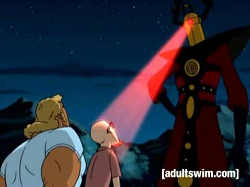
\includegraphics[width=\figwidth]{pics/11/18.png}
	\end{center}
\end{wrapfigure}
Instead of an explosion of angry binary or an immediate attack, the awkward silence was broken by a second voice exploding into laughter. 
It wasn't exactly happy laughter: 
it had a definite hysterical edge to it and went on for far longer than Tink's comment warranted. 
As we sat and waited for it to peter out Sarge cut his comm and asked Twitch if he recognized the voice. 
Both of them agreed that the speaker was female and someone they'd met before, but couldn't pin it down. 
Sarge was on the edge of interrupting and asking for some identification when the tech-priest commanded the woman to "Cease her frivolity." This did not go over well.

You know how some people argue like an old married couple and it's sort of cute to watch? 
Well this wasn't anything like that. 
They argued like, well, two people who'd been stuck on a desert island together for far too long. 
Or one person and one damaged blender. 
It wasn't just awkward to listen to, it was actually a little scary. 
Weeks or months of pent-up venom poured out in a nearly-incomprehensible tirade from the woman and the priest countered with commands for silence and bursts of binary. 
It only got harder to listen to when the cogboy cut his comm and she left hers on.

Now that she was talking most of us recognized the woman's voice and at Sarge's order we followed the sound of the argument. 
After a few blocks of walking we found a familiar guardswoman, face gone crimson, screaming at a senior-looking tech-priest. 
They were standing in the middle of a half-looted convenience store with half a dozen servitors forming a menacing looking ring around the woman. 
Nubby and Twitch grabbed Tink before he could anything stupid and Sarge awkwardly cleared his throat.

To everyone's surprise, especially Sarge's, the argument came to a sudden halt. 
Our fearless leader was nearly knocked off his feet as the guardswoman screamed his name and tackled him. 
Nubby took a picture.

\begin{wrapfigure}{O}{\figwidth}
	\begin{center}
		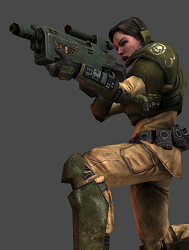
\includegraphics[width=\figwidth]{pics/11/19.png}
	\end{center}
\end{wrapfigure}
While being tackled by a heavily armed and moderately attractive woman is surprising in its own right, what really caught us off guard was the fact that she was crying. 
See, we knew this guardswoman, both as a fellow passenger from the Occurrence Border, and as one of the few survivors of a rather unsuccessful mission to purge some genestealers. 
She was originally from some nobby regiment and had one of those thirty syllable names, but we all called her Aimy.

Now, if any of us had been asked to describe Aimy we'd have used words like Solid, Professional, and Dangerous. 
Never hysterical or weepy or inclined-to-hug-random-noncoms. 
I mean, it was a commonly held belief that she'd saluted her own mother every night before bed. 
Which sort of made sense when you remembered that her mother was a Lord General. 
Anyway the point is that her breakdown was terrifying more than anything.

Sarge disentangled himself and, as politely as possible, asked Aimy why the hell she was here. 
Last any of us heard her team had been farther towards Tau space and had been one of the ones to go MIA. 
Nubby chimed in and pointed out that everyone had thought she was dead. 
Twitch suggested that maybe she was, and asked Fumbles to check if she was a ghost. 
This triggered another round of hysterical giggling and got Twitch a hug of his own, which terrified the demolitions trooper.

The reunion was brought to a halt when the tech-priest rolled over to us with his servitor posse. 
In typical high-ranking cogboy fashion he commanded everyone to shut up and take him to the shuttle. 
Our presence was not ideal, but could be made to serve the Omnissiah. 
This triggered another shift from hysterical to furious in Aimy.

\begin{wrapfigure}{O}{\figwidth}
	\begin{center}
		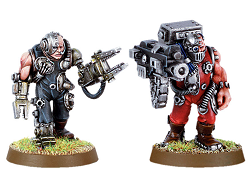
\includegraphics[width=\figwidth]{pics/11/20.png}
	\end{center}
\end{wrapfigure}
This time we were in a better position to understand what was being said. 
The main thread of the argument seemed to be that the Magos had gotten everyone killed, refused to call for a pickup, and gotten them stranded on an empty world for his bloody metal god. 
Aimy was done serving the Omnissiah.

For his part the cogboy, who Sarge finally recognized as the xeno-tech hunting Magos who'd been part of our expedition, turned his vocoder up to maximum volume and tried to counter each individual point. 
Why he was doing it was a mystery, because everything he said just made Aimy angrier and convinced us that the guy was a complete tool. 
The bullshit about how his mission couldn't be jeopardized by bringing in unbelievers or how he was not responsible for the behavior of organics was bad enough, but the crowning moment of tool-dom was when he pointed at three familiar looking servitors and claimed that Aimy's companions "still retained the majority of bodily functions." That neatly answered the question of where the arbite and clerics she'd been teamed up with had gotten to.

Over the next few minutes things degraded even further as Tink started needling the tech-priest as well. 
Sarge was about ready to step in and end the shouting match one way or another when Twitch sidled up next to him. 
In the quietest and calmest voice he could manage, Twitch told Sarge that these guys weren't the movement he'd spotted and he was fairly sure we were being watched. 
He asked if we could, very casually, start falling back to a more defensible position. 
Sarge looked around at the floor to ceiling windows on three of the walls around us and agreed that that might be a good idea.

\begin{wrapfigure}{O}{\figwidth}
	\begin{center}
		
\includegraphics[width=\figwidth]{pics/11/21.png}
	\end{center}
\end{wrapfigure}
Employing the entirety of his acting talent, Sarge announced that some fresh air might calm everyone down. 
Nubby took the hint and grabbed Aimy while Sarge tried to chivy the Magos out of the shop, when that didn't work he just got behind the tech-priest and started pushing until he got the point. 
Twitch, trying to keep his head from swivelling like a nervous pidgeon's, set his eyes on a sturdy looking garage and led the way

Twitch casually gave a hand signal as he walked. 
Tink correctly interpreted this as an order to send out his stealthed drone and Fumbles got the point after Nubby kicked him in the shin. 
The psyker swayed a little and tripped over a curb, but when we hauled him to his feet he shook his head and muttered about everything looking clear.

At the back of the group the shouting match continued, even though Aimy's heart obviously wasn't in it anymore. 
She'd picked up on what was happening and everyone could tell she was trying to hide the fact that she was terrified. 
The only people that were oblivious to the change in the atmosphere were the tech-priests. 
The Magos had really started picking up steam now that Aimy was distracted; 
he was loudly badmouthing just about everyone and made it very hard to concentrate on looking casual.

We'd reached the edge of the garage when Tink made a sort of high pitched wheezing sound and went pale. 
Everyone took the hint and started power-walking towards the opening. 
Well, almost everyone. 
At the back of the group the Magos and his servitors had come to a halt and the tech-priest was in full monologue mode. 
He stood there, stock still and surrounded by his herd of servitors, and loudly declared his genius, devotion, and general craziness to the rest of the world. 
As he entered the safety of the garage Sarge glanced back at the Magos then at Tink, who shook his head violently.

Sarge sighed, grabbed a smoke grenade, and chucked it at the Magos' feet at the exact same moment the sniper fired.

\begin{wrapfigure}{O}{\figwidth}
	\begin{center}
		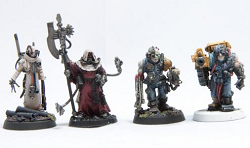
\includegraphics[width=\figwidth]{pics/11/22.png}
	\end{center}
\end{wrapfigure}
The shot was perfectly aimed: 
a nearly invisible las-beam of came in at the Magos' eye level. 
It would've been a clean kill if he hadn't had a refractor shield. 
There was a blinding flash where the beam met the shield and the tech-priest started screaming orders at his servitors. 


Now that the charade was over Sarge asked for a sitrep as everyone got their weapons ready. 
Tink claimed there were two hostiles wearing some sort of stealth suits and carrying rifles, neither of them had line of sight inside the garage. 
Their stealth was damned good, so there were probably more he hadn't spotted, but they either couldn't hit us or were all focusing on the Magos. 


Speaking of the Magos, he'd apparently decided not to come join us in our cover and had hunkered down in the smoke with his servitors. 
The six meat-puppets had formed a sort of wall around him and were firing an indiscriminate barrage into the surrounding area. 
It didn't look like they had any real idea of where the snipers were and as we watched two of the servitors went down to incredibly well-placed shots. 
Our desire to go out there and help him dropped sharply.

All of us were familiar with sniper and counter-sniper tactics. 
Tink was told to continue sweeping for hostiles and Fumbles was ordered to do likewise. 
The theory was that once we had their location we could lay down suppressing fire or start flanking. 
Until we knew where all the snipers were, even if none of them had shot at us yet, we were effectively pinned. 
Unfortunately, something about these hostiles had Fumbles stumped he could barely even locate the ones Tink had spotted. 
The little guy gritted his teeth and pump more psyk into his detection field, but we all felt a wave of despair from him as he only succeeded in covering himself in painful sheet of static-electricity. 


Outside another servitor dropped to a head-shot and the Magos started yelling at us to help him.

\begin{wrapfigure}{O}{\figwidth}
	\begin{center}
		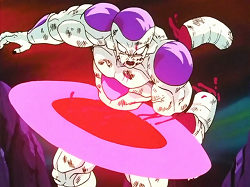
\includegraphics[width=\figwidth]{pics/11/23.png}
	\end{center}
\end{wrapfigure}
It was officially time to either shit or get off the pot, at the current rate the Magos was going to be dead before we had all the snipers localized. 
The more pragmatic members of the squad pointed out that this wasn't such a bad thing and suggested that we just run for the shuttle while he drew fire, but Sarge vetoed this perfectly valid plan. 
At his order everyone popped smoke and split out in two teams. 


Sarge, Aimy, and Twitch pushed out and started laying suppressive fire and grenades onto the two rough locations Tink had given them. 
Tink, Nubby, and Fumbles went out the back to try and flank the sniper between us and the shuttle. 
Meanwhile, Jim ordered his three skulls to help the drone search the area, warmed up the shuttle's perimeter defences, and relayed the situation to the ship.

Everything started out so well. 
The two snipers immediately stopped firing, Tink managed to spot a third and put a plasma-bolt through the bastard's cover, and our flankers were almost in position. 
It was really looking like we were going to be able to neutralize the hostile or at least get to the Magos and start a nice, orderly retreat. 
Then two things happened and everything went to shit.

At first we thought the snipers had popped smokes of their own and were falling back. 
The buildings they were holed up in went sort of hazy and vague, but the fog didn't drift and a second later the snipers resumed firing from inside the cloud. 
Another servitor went down and Twitch's grenade detonated in mid-arc. 
Fumbles screamed "PSYKER" at the exact same moment the lascannon fired.

Lascannon really isn't the right world, but damned if we could think of a better one. 
A lascannon typically fires a large, powerful beam, and brief beam. 
This thing was barely larger than a multi-laser and walked in a brief arc across the battlefield. 
It just sliced through everything it touched: 
walls, lampposts, the car Sarge was hiding behind, servitors, and tech-priests.

\begin{wrapfigure}{O}{\figwidth}
	\begin{center}
		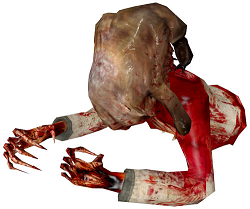
\includegraphics[width=\figwidth]{pics/11/24.png}
	\end{center}
\end{wrapfigure}
Sarge laid there for a second, trying to blink away the purple afterimages and get his bearings. 
He was lying on the ground and was also apparently inside of a car. 
He looked out a side window, which was oddly level with his head, and saw some sort of red and chrome spider monster flailing towards him. 


Sarge tried to turn his lasgun towards this new threat, but it was wedged against the roof of the car. 
He futilely pushed at the roof with his hands, then his legs, as the spider thing inched closer on it's metal legs. 
At the last second a pair of hair-thin beams stabbed into the spider and it fell to the ground. 
Sarge breathed a sigh of relief which turned into a choked scream when something tightened across his throat.

Twitch hauled Sarge out from under the decapitated car by the collar. 
It was an impressive feat given their relative sizes and the unhelpful way the big man was flailing around. 
The servitors were scragged, those last sniper shots seemed to have finished off the cogboy, and there was no telling what the psyker or lascannon would do next. 
In his professional opinion it was time to live to fight another day.

Twitch hit Sarge with his emergency stimm while Aimy popped her last smoke. 
Under its cover they half-carried Sarge back to the relative safety of the garage. 
Once inside, Aimy kept her longlas trained on the smoke-filled entrance while Twitch tried to fill everyone in on the situation. 
Before he got two words out the lascannon cut through the entire building at shoulder height.

\begin{wrapfigure}{O}{\figwidth}
	\begin{center}
		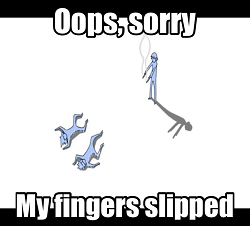
\includegraphics[width=\figwidth]{pics/11/25.png}
	\end{center}
\end{wrapfigure}
The flanking team was having better luck all things considered. 
Jim's skulls were hounding the sniper Tink had flushed out and Fumbles had a rough bead on the enemy psyker. 
Tink sent his drone to get the exact position and charged up his plasma-gun while Nubby and Fumbles poured las-fire and psychic shrieks into the clouds concealing the two active snipers. 
Their accuracy was abysmal, but the angle of their attack and sheer volume of fire was enough to force the hostiles to rebase. 
None of them realized how bad the situation had gotten until they heard Twitch's warning get cut off by the second lascannon strike.

In an uncharacteristic act of bravery Nubby led the charge back towards the garage, taking Fumbles with him and leaving Tink on overwatch. 
Jim diverted his medi-skull to follow them, then sent the rest of his minions to find the lascannon before it could fire again. 
They found the building teetering alarmingly, but still upright and with Sarge standing in the middle, barking at the other two troopers to get back on their feet.

Back in the garage Sarge was dealing with a minor mutiny. 
He was of the opinion that Magos was still alive and a pickup needed to be made, Twitch and Aimy disagreed. 
Nubby got to the door just in time to hear the noncom shout that the Magos was still moving and could be saved if they hurried. 
Aimy countered this argument by hefting her long-las and putting a hot-shot through the head of the twitching tech-priest. 
Further debate was delayed by the roof caving in.
\begin{wrapfigure}{O}{\figwidth}
	\begin{center}
		
\includegraphics[width=\figwidth]{pics/11/26.png}
	\end{center}
\end{wrapfigure}
There's nothing like a few tons of collapsing stone to motivate a hasty retreat. 
Nubby, as usual, led our sprint back to Twitch's position with a stimmed up Sarge hard on his heels and the rest of the group trailing behind. 
None of us even registered Jim's question over the comms.

As we regrouped Tink's drone finally found his target, a large blob of overcharged plasma sailed across the plaza and into a tasteful little restaurant. 
Instead of just burning through the building it splashed against something in the back with a crackling explosion. 
Tink cheered, then swore, then yelled something about tackle and burst into laughter. 
Twitch barely managed to pull him down in time: 
the sniper's shot cut a neat little notch out of the techie's helmet.

None of us wanted to start this shit again. 
Fumbles threw up a half-assed cloak, and we all started falling back towards the shuttle in pairs. 
Now that we knew what to look for we could see three indistinct blurs poking in and out of cover, we did our best to return fire as we ran, but the buggers had nerves of steel. 
For every ten shots we put down range they returned one incredibly well aimed one. 
Only the combination of our cover, Fumbles' cloak, and a huge amount of suppressive fire kept us alive.

That's not to say we got out of there unscathed, those hair-thin las-bolts nailed everyone at least once. 
If you stuck a toe outside of cover they'd shoot it, and if you didn't they'd try and punch a shot right through. 
The only one of us who managed to score a hit on them was Aimy, and the second time she tried to line up a shot her long-las exploded in her hands as they put a shot down the barrel. 
Stopping and waiting for Jim's medi-skull, which had gone Emperor-knows-where during the retreat, was out of the question, so Sarge wound up popping another stimm and carrying her for the last sprint to the shuttle. 


We all felt tremendous relief when the shuttle's multilasers finally forced the snipers to back off.

\begin{wrapfigure}{O}{\figwidth}
	\begin{center}
		
\includegraphics[width=\figwidth]{pics/11/27.png}
	\end{center}
\end{wrapfigure}
As we reached the top of the shuttle's loading ramp Twitch asked if anyone knew what had happened to the lascannon. 
Right on cue a section of bulkhead started glowing then the damned beam punched through with a spray of molten metal. 
Jim didn't bother waiting for an order, the engines roared to life and our big, ungainly shuttle started to wallow upwards. 
As the rear ramp began to close the lascannon fired again and neatly burned through its hydraulics. 
Everyone resisted the urge to go poke their heads out the broken door and see what was shooting those beams at us.

At this point Tink, who'd been rather focused on not getting shot like the rest of us, realized that someone was missing. 
He yanked the drone controller off his harness and started screaming at Jim to slow down. 
Jim correctly interpreted this as a terrible idea and ignored it. 
Everyone who wasn't collapsing from blood loss or stimm aftereffects watched as the techie frantically slammed at the drone's controls and screamed curses. 
The show was briefly interrupted when the lascannon burned through the floor about a meter in front of Tink's feet, but resumed after a few evasive maneuvers slammed us around like pinballs.

It didn't take a savant to see that Tink was losing his race. 
Spot the wonder-drone was great at stealth and recon, but it just wasn't built for this sort of speed. 
Nubby clomped over and put a hand on techie's shoulder. 
He suggested that maybe Tink should park the drone somewhere, we'd probably be able to come back and get it in a few years.

Tink whirled around and had his drone controller raised like a club when the lascannon fired again. 
The shuttle pitched forward as the tail of the vessel exploded in a fireball.

\begin{wrapfigure}{O}{\figwidth}
	\begin{center}
		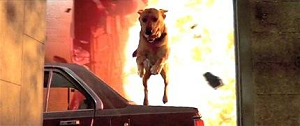
\includegraphics[width=\figwidth]{pics/11/28.png}
	\end{center}
\end{wrapfigure}
The difference in attitude between Tink and the rest of us when the lascannon took out our tail engine was profound. 
While everyone else screamed, clutched at the safety handles, or prayed to the Emperor, he let out a whoop of joy and ran to the jammed ramp. 
A few sniper beams sailed past him and were ignored in favor of a small tan shape which, now that our speed had been cut in half, was steadily growing larger.

Tink cooed at the damned thing like a puppy, which was admittedly better than a girlfriend, but still. 
As it closed the last dozen meters he spread his arms wide and tried to catch it, only to get knocked off his feet as a smaller and faster object sailed through. 
The drone followed a second later and slammed into Twitch, who'd been holding on for dear life in a far corner.

Tink sat up and groped at the object that had knocked him on his ass. 
He raised two blood-covered hands, registered that he was holding a severed head attached to a medi-skull, and started screaming. 
Jim appeared in the hatch leading to the cockpit asked if the magos had made it aboard. 


The cogboy barely managed to wrench the gorey thing away from Tink before it was chucked back out the tail hatch. 
Jim held the Magos' head up like some sort of trophy and turned to face Sarge with a rather proud expression on his face. 
Unfortunately our barely conscious leader wasn't able to offer any suitable praise, all he managed was bleary "Who's flying the shuttle?"

Jim swore and ran back into the cockpit, barely managing to dodge the next lascannon beam. 
Thankfully that was the last shot, everyone breathed a sigh of relief and slumped into their seats. 
Well more of a gasp of relief, we were all pretty out of breath and our ears were hurting for some reason. 
Tink eyed all the holes in the cargo-bay and kicked the rest of us to our feet.

We wound up packing seven people and, for some damned reason, the drone into the two-man cockpit. 
It wasn't comfortable, but at least there was air.

\begin{wrapfigure}{O}{\figwidth}
	\begin{center}
		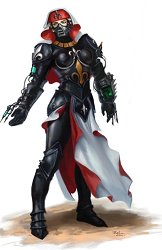
\includegraphics[width=\figwidth]{pics/11/29.png}
	\end{center}
\end{wrapfigure}
Between all the sweating, bleeding people, the Magos' severed head, and Nubby's uniquely indescribable odor that cockpit was getting pretty manky by the time we reached the Occurrence Border. 
As soon as the bay was pressurized we piled out and collapsed on the first available surface. 
The ship's air, which always smelled faintly of burnt cabbage, had never tasted so sweet.

The Hospitaller and her minions were waiting for us in the docking bay along with a disconcertingly high number of tech-priests. 
Thinking fast, if not hard, Tink jammed the techno-heretical drone up the front of his shirt, which made him look pregnant and caused a fair bit of amusement among the orderlies. 
None of the cogboys seemed to notice, and after they'd taken possession of the Magos' head, for Data Extraction they'd said, all of them left without incident. 
Sarge tried to follow them, but only got a few meters before the Hospitaller neatly tripped him onto a gurney. 
The incredibly fluffy pillow defeated any further attempts to refuse treatment.

While the burns Aimy had received when her long-las exploded got the most attention, all of us wound up getting hauled to the medbay by Doc's valkyrian girlfriend. 
Well, except for Jim, who tagged along with the other tech-priests to keep an eye on his… sample? 
trophy? 
rescuee? 
Whatever you called the head your medi-skull had sawed off the still-warm body of its patient. 
Seriously, that right there is why no one trusts those things.

\begin{wrapfigure}{O}{\figwidth}
	\begin{center}
		
\includegraphics[width=\figwidth]{pics/11/30.png}
	\end{center}
\end{wrapfigure}
Anyway, everyone except Sarge was stuck in the medbay for a while. 
Despite their size, those sniper beams had been just as nasty as any lasgun's, and it was surprising how many holes we had in us. 
Sarge was set loose after a basic patch-job and yet another stimulant, thankfully not a combat one this time, to go and talk with the adepts and other Interrogators. 
Doc made him promise to come back for a complete round of treatment the second the situation was resolved.

Speaking of Doc, he was rather happy to see us all again. 
Nubby filled him in on the basics of what had happened, with Twitch and Fumbles correcting the occasional exaggeration. 
Doc was as surprised as the rest of us had been when we got to the part about running into Aimy and the Magos, he wheeled over to where she was being treated by the Hospitaller just to verify we weren't bullshitting him. 
In his semi-professional medical opinion she was in for a rough few days as they speed-grew the skin on her face and arms, but she should recover without much scarring or needing any augmetics. 
He claimed his girlfriend had a lot of experience treating burns, something about working with trainee dominions.

While the rest of us chatted with Doc, Tink had pulled the screen around his bed and loudly threatened to shoot anyone who looked inside. 
Occasionally the nurses would look up at the loud clanging sounds and the Do Not Disturb sign then start giggling. 
When the humor of the situation wore off and the noise was starting to get really annoying, we steeled our nerves and went to see just what he was doing in there. 


\begin{wrapfigure}{O}{\figwidth}
	\begin{center}
		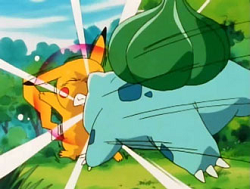
\includegraphics[width=\figwidth]{pics/11/31.png}
	\end{center}
\end{wrapfigure}
We found Tink with the drone between his legs, but thankfully his pants were on. 
He was trying to pop out an impressive dent in the front of Spot's chassis. 
When asked how it'd happened he reminded us of the enemy psyker he'd taken out. 
It'd used some sort of shield to deflect his plasma bolt and looked like it was about to launch its own attack. 
So he'd had Spot ram the bastard, it's hard to cast spells when fifty kilos of angry drone is bashing your head in.

Turns out the psyker had one hell of a helmet though, hence the dent. 
Still, it'd convinced the warpy bastard that it was time to fall back, so he was calling it a win. 
Doc, who'd been eyeing the large lens next to the dent, cut into the story at this point and asked if that meant he had a clear picture of the attackers. 
Tink shrugged and admitted that he probably did, but so did the adepts who'd been watching the feed. 
They'd get around to telling us tell us who it was eventually and he was the only one who could fix this dent, so his priorities were clear. 


The rest of us were a little more curious so Nubby yanked the spanner out of Tink's hands and refused to give it back until he pulled up the vid of the ramming. 
After a little fast-forwarding he found it and everyone crowded around the data-slate. 
We were treated to a view of a small room with a blurry figure standing in the middle of it and gesturing. 
As we watched the blur was replaced by a large circular shield and the screen went blindingly bright. 
When the flash faded there was a tall robed figure with a sword and egg-shaped helmet standing there panting. 
He raised his sword, gathered some sort of lighting around it, and then the drone hit him right in the back of his stupid hat.

\begin{wrapfigure}{O}{\figwidth}
	\begin{center}
		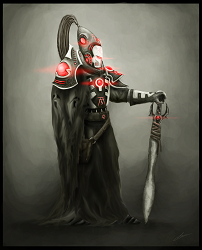
\includegraphics[width=\figwidth]{pics/11/32.png}
	\end{center}
\end{wrapfigure}
Other Inquisitorial agents might have sat there and carefully examined the psyker's robes or weapon for clues. 
We just kept having Tink rewind it so we could see the headbutt again. 
When he got the sound turned on it made this great sort of hollow clang every time the drone hit him. 
There was much debate over which was the best part, the initial impact or the part where his head went through the drywall and got stuck. 
Either way it was the best show we'd seen in a long time

We wound up putting the vid on repeat on all the screens in the medbay. 
It was very therapeutic to see the bastard flailing his fancy sword around in an attempt to fend off the drone and cut his head free at the same time. 
At Twitch's urging Tink even etched a little egg-helmeted face on the side of Spot's chassis to commemorate the event. 
Everyone was in remarkably good spirits considering we were stuck in the medbay for the foreseeable future. 
Well, except for Aimy who was still tranqued up for the worst part of her burn treatment. 
Fumbles tried to send her a mental image of the whole thing as she slept, but Doc made him stop after a nearby diagnostic cogitator caught fire.

While the rest of us were laughing ourselves sick over the Inquisitions Funniest Home Videos, Sarge was attending a very serious meeting with some very serious people. 
You could tell they were serious because none of them even smiled when the adepts played the drone-ramming clip for them; 
they just muttered to each other about which craftworld the Eldar Warlock had come from and what possible hand they could have in everything. 
Sarge primarily contributed to this discussion by resting his head on the table and agreeing with anything our team's adepts said.

\begin{wrapfigure}{O}{\figwidth}
	\begin{center}
		
\includegraphics[width=\figwidth]{pics/11/33.png}
	\end{center}
\end{wrapfigure}
In Sarge's opinion the other two Interrogators were putting way too much effort into trying to understand the Eldar's motives. 
They'd gone through the vids from Tink's drone and Jim's skulls frame by frame and determined that there'd been a Warlock, three rangers, and some sort of heavy weapon team operating a brightlance. 
There was a little debate on the last point, since all of Jim's drones had been shot before they could get a good picture. 
Neither of the other teams had run into any hostiles, and they hadn't spotted anything when they'd done a flyby of the island, so it looked like that was it for their ground assets.

Sword-guy halfheartedly suggested that the Eldar could be behind the disappearances, they were xenos with access to warp powers and archeotech after all. 
He didn't press the issue when Sarge grumpily asked why they hadn't used their creepy-silhouette-leaving people-disappearer instead of shooting at us with fancy lasguns.

Battleaxe claimed that the small size of their force suggested they were an assassination team. 
Given their attack pattern, location, and the fact that no one else of importance was nearby, their target must have been the Magos. 
From his spot at the end of the table Sarge grumbled that he'd told everyone the xenos had been trying to kill the tech-priest an hour ago. 
Battleaxe ignored him and pointed out that the real question was whether this was connected to the disappearances and if it was because Magos had known something. 


Rather annoyed at having been ignored, Sarge sarcastically suggested that they ask the Magos that question. 
To his considerable surprise everyone took this seriously, with Sword-guy even asking his psyker if he was capable of leading a seance. 
The debate over whether the ritual was more likely to result in useful information or a daemon manifestation was still raging when the tech-priests arrived.

\begin{wrapfigure}{O}{\figwidth}
	\begin{center}
		
\includegraphics[width=\figwidth]{pics/11/34.png}
	\end{center}
\end{wrapfigure}
Just saying they arrived doesn't do it justice. 
Every single cogboy over the rank of Enginseer on the Occurrence Border walked, rolled, floated, or slithered into the meeting room. 
The ratio of metal to meat in there hit fifty-fifty in the first few seconds and climbing towards eighty-twenty when Jim brought up the rear of the procession. 
Sarge took notice of how nervous the younger cogboy looked as, at an order from a senior tech-priest, he sealed the door behind him. 


It occurred to the burly noncom that if a bunch of Guardsmen had done something like this, it would've been because some officer was about to become a friendly fire statistic. 
Sarge edged his chair away from the table and towards the most defensible corner he could find and casually put one hand in his pocket. 
No one except Jim paid him any attention. 
The Enginseer leaned out from behind his seniors and awkwardly tried to indicate that this was not the time to pull out a grenade. 
Or possibly that his neck hurt and he wanted to lie down for a while, Jim was bad at Guard hand signals.

After a bit of unpleasant silence the coggiest of the cogboys finally decided that the tension had built to acceptable levels. 
In a loud, authoritative, and entirely synthetic voice he proclaimed that a seance would not be necessary, they'd extracted all relevant data from the Magos' eidetic memory chip. 
He just sort of stopped there with no explanation of what the data actually was, leaving the non-metallic portion of the room awkwardly waiting. 
The second Battleaxe began to ask, the head tech-priest cut her off with a shout of "That information is sacred. 
It contains Mechanicus secrets. 
Sharing it with the those who do not venerate the Omnissiah in his true form would be heretical." The cogboys behind him echoed the words Sacred, Secrets, and Heretical like shitty backup singers.

Sarge let out a weary sigh and rubbed his aching temples. 
It was going to be a long meeting.
\begin{wrapfigure}{O}{\figwidth}
	\begin{center}
		
\includegraphics[width=\figwidth]{pics/11/35.png}
	\end{center}
\end{wrapfigure}
When Sarge finally staggered back into the medbay he looked bloody exhausted. 
He pretty much collapsed in the first available bed and at his request we stopped the continuous loop of the Warlock getting his head stuck in the wall. 
Doc gave him some overdue medical treatment he filled us in on the situation.

To start with, he gave us the official word that we'd been shot full of holes by an Eldar hit-squad. 
Nubby fistpumped and loudly started calculating what his and Fumbles' share of the pool was. 
Sarge immediately crushed this happy speculation with the news that the Eldar weren't the cause of the attacks, and had only been there for the Magos unless Aimy could tell us otherwise. 
No one would be collecting on the pool anytime soon and, unless there was a second group of Eldar, Nubby's odds weren't looking good.

While Nubby whined to himself the discussion shifted to the Magos, his decapitation, and the tech-priests. 
According to Sarge all of them, even Jim, had a gear up their ass about something they'd gotten out of the Magos' head. 
It'd been like pulling teeth to get anything out of them, they kept falling back on the whole "We technically only have to answer to the Inquisitor so get an order from him" arguement. 
In end all they were willing to part with was that the Magos had been chasing a piece of archeotech and had tracked it into the xeno territory. 
He'd intercepted some reports that confirmed that nature of the archeotech and the heresies the xenos had committed on it. 
He'd then sent a report to the PROPER AUTHORITIES and was still tracking the archeotech when he was killed by the vile Eldar. 
Finally, the nature of the tech was not for us to know, but it would not cause the sort of disappearances we'd seen; 
we should turn our investigations elsewhere.

The priests had refused to say anything more. 
The PROPER AUTHORITIES had been notified and the matter should be left to them. 
Further probing into the Mechanicus' holy secrets would be unwise.

\begin{wrapfigure}{O}{\figwidth}
	\begin{center}
		
\includegraphics[width=\figwidth]{pics/11/36.png}
	\end{center}
\end{wrapfigure}
It had taken a heroic effort by the other two Interrogators and our old diplomat adept to convince the tech-priests that their warning was understood. 
The entire army of cogboys had left secure in the knowledge that no one would be poking into their business, and that everyone would be focussing on the completely unconnected matter of the disappearances. 
The second they were gone one of the psykers had done something that made the room sound all weird and the diplomat had asked for a show of hands. 


"Who here," he'd asked, "thinks we're looking for a piece of insanely dangerous archeotech, that's either wiping all intelligent life off worlds or is being pursued by someone who is willing to do so to keep it secret." The Ayes had it by a landslide; 
Sarge said it was nice to be reminded that not everyone in the Inquisition was stupid or insane.

In the end the working theory was that someone was hauling this thing from Tau space to the Imperium via warpship. 
Whether it was to sell, study, worship, or use as a weapon on Imperial worlds was up to debate, but it was obvious that the Mechanicus and the Eldar were both chasing it. 
It was impressive that whoever was carrying it was managing to stay ahead of both of them, the fact that they were evading pursuit probably explained the semi-random course across the the border worlds though.

The question was what to do about it. 
There was no way we'd back off and let the Admech handle things, Imperial worlds getting wiped out like the one we'd just visited wasn't acceptable. 
The only options were to try and catch the carrier in a stern chase, try to predict their next destination and set an ambush, or go get some real reinforcements and try to lock down the entire sub-sector. 
Debates were had, charts were consulted, the Captain was called down, and three possible destinations were laid out.

\begin{wrapfigure}{O}{\figwidth}
	\begin{center}
		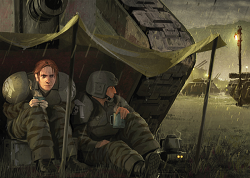
\includegraphics[width=\figwidth]{pics/11/37.png}
	\end{center}
\end{wrapfigure}
The Captain was in favor getting reinforcements and wanted us to chart a course to the largest Imperial world along the border. 
Battleaxe and Sword-guy thought too much damage would be done before a response was mustered. 
She wanted us to try and jump ahead to a refueling way station that looked like it might be in the right direction; 
he wanted to head towards a nearby Imperial world with a rather untrusted governor that might be either be a target or buyer. 
Sarge, who was barely awake enough to follow what was going on, wound up being the tie-breaker.

When all three of his adepts had just shrugged, Sarge had fallen back on his noncom instincts. 
He'd stood straight, squared his shoulders, and stabbed his finger at the middle option on the chart. 
Sarge'd loudly declared that it was the only real choice, then retreated back up to the medbay before anyone realized he'd just randomly picked one. 
None of us saw any problem with this decision making process.

In the morning, or whatever you call it when the ship's lights jump from ten percent to max power and the Captain blares reveille over the comm system, Sarge got around to debriefing Aimy. 
She told a fairly unpleasant tale of wandering around the ass-end of the sector as the Magos did his thing. 


Aimy and her team had been treated like mushrooms, that is to say kept in the dark and fed horseshit. 
They'd never learned anything about their mission aside from the fact that archotech was involved, and had mostly spent their time getting shot at by over a dozen different groups ranging from gangers to planetary police forces. 
It wasn't some sort of giant conspiracy though, the Magos just didn't give a shit; 
If there was something in the way he'd throw bodies at it all day long if it meant getting through quicker. 
He wasn't too particular about where those bodies came from either, if his team couldn't handle a problem he'd improvise. 
Aimy claimed she'd never look at servitors the same way again.

\begin{wrapfigure}{O}{\figwidth}
	\begin{center}
		
\includegraphics[width=\figwidth]{pics/11/38.png}
	\end{center}
\end{wrapfigure}
The next to last straw for Aimy had been an ambush by what she now recognized as Eldar. 
That'd killed off the last of her teammates and forced a retreat onto a merchant vessel. 
The Magos had then proceeded to intimidate and bully the merchants into taking him on a tour of the empty worlds. 
To no one but the Magos' surprise, that relationship had ended with the merchants ditching them at the first opportunity, hence the island. 


She'd been stuck there alone with him, well him and the servitor converted bodies of her teammates, for a month. 
The real kicker was the bastard had a sort of interstellar communicator the whole time. 
He'd used put in a call to the nearest Forge World but had refused to contact anyone else after the merchant incident. 
So yeah, all that went a long ways to explaining the hysterics and head-shooting incident. 


The end of story though, was Aimy had no really new intel. 
Between obvious clues, well obvious to our adepts, and that incredibly unsubtle warning from the cogboys, we knew just as much as she did. 
Speaking of that warning, it'd been awfully convenient that the tech-priests had decided to give it to us instead of just staying quiet. 
We all suspected that Jim and Hannah had had some hand in the matter, but neither of them were talking to us currently. 


As the least-shot member of the squad Nubby, and by extension Fumbles, had been sent to chat with two junior tech-priests after they didn't visit us in the medbay. 
When Nubby returned he claimed that every time he'd tracked one of them down they'd gotten these really nervous expressions and ran for it. 
He'd given up after Jim had locked him and Fumbles in a section of maintenance corridor. 
Also, if Ol' Bill came by asking why one of his techs had a massive headache and why there were reports of warp-ghosts on deck eight, that had nothing to do with him or Fumbles getting tired of waiting for the doors to open again.

\begin{wrapfigure}{O}{\figwidth}
	\begin{center}
		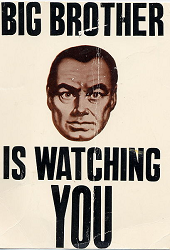
\includegraphics[width=\figwidth]{pics/11/39.png}
	\end{center}
\end{wrapfigure}
The destination Sarge had chosen, which turned out to be the way station, was a solid week of warp travel away. 
After about the second day everyone was tired of sitting around the medbay with Doc and his ladyfriend, so we moved back to our nice Gellar Field Generator adjacent quarters. 
Doc complained a little that our treatments, especially Aimy's, weren't finished, but we figured that coming down and making a few housecalls would be good for him. 
He'd been getting soft being in that chair all day, some exercise would do him good.

Sarge spent most of the next week putting together reports and contingency plans with the adepts and Interrogators, but he spared some thought for Jim and Hannah. 
He'd interpreted the junior tech-priests' behavior as a sign that their bosses were acting crazier than usual over this whole thing, and made a note to keep an eye on them. 
Intimidating impressionable young tech-priests was OUR shtick. 
Since sending Nubby, Twitch, or Tink to watch them was likely to do more harm than good, some words were had with Ol' Bill and the Captain. 
The duty roster was shuffled and several unintrusive armsmen and engineers were assigned to the same shifts as our cogbros. 
It might have been a bit of a paranoid over-precaution, but that's sort of what being a guardsmen in the Inquisition is all about.

Nubby and his partner in petty-crime wandered around the ship a lot during our transit. 
Anyone with enough brains to pour water out of a boot could tell they were planning to sabotage the betting pool in some way before their inevitable loss, but it wasn't worth doing anything about. 
As long as Nubby didn't egg Fumbles into changing someone mind for them again, it was about as harmless a pastime as they were likely to find.
\begin{wrapfigure}{O}{\figwidth}
	\begin{center}
		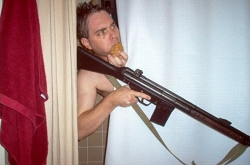
\includegraphics[width=\figwidth]{pics/11/40.png}
	\end{center}
\end{wrapfigure}
Aimy, who was doing pretty well despite having bags of medical gel stuff taped to half her face and one hand, had initially moved back into the quarters where her team had stayed. 
Unfortunately, those rooms brought back some unpleasant memories and she was pretty sure the tech-priests were following her. 
She said that every time she'd turned there was a servo-skull or servitor working nearby. 
Twitch sympathised with her and offered a solution. 
He proudly explained that our little base was 99% servitor free, and that other 1% would be gone when he found a ladder tall enough to reach the chunks that had stuck to the ceiling. 


She accepted of course, how could anyone refuse an offer like that? 
About an hour after Aimy moved in her suspicions about the servitors were proved correct when the door claymore gibbed a cleaning servitor. 
Twitch immediately replaced the mine and got another kill within ten minutes, though that one might have just been there to clean up the first. 
Either way, they stopped coming after that and Aimy settled into Doc's section of room. 
She became about as much of a shut-in as Twitch, splitting her time between sleeping off her medical treatment and playing with the toy Tink gave her.

\begin{wrapfigure}{O}{\figwidth}
	\begin{center}
		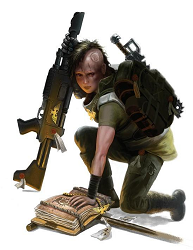
\includegraphics[width=\figwidth]{pics/11/41.png}
	\end{center}
\end{wrapfigure}
Tink and Twitch's lives over the week generally revolved around our new barracks-mate. 
Tink, who seemed a little lonely now the Jim wasn't there to argue with him, had fixed Spot's chassis and replaced it's servo-grox-skull disguise before the end of the second day. 
After that he went back to work on the xenos pulse rifle camouflage project and seized on Aimy as a guinea pig. 
She was in the market for a new weapon after all, and it was so much easier to cram a pulse rifle into a long-las' chassis than a regular lasgun's. 
They spent quite a while blowing holes in various objects and badmouthing tech-priests. 


Twitch was just glad to have an actual reason to distrust the servitors and turned the barracks' defences up from 11 to about 13. 
Sarge called for a slight de-escalation when he started putting small remote charges on every servitor he encountered, just in case they turned en masse. 
Apparently Jim and Hannah were the ones who had to find and defuse them.

On the seventh day Sarge and the other Interrogators put everyone on an hour alert and prepped the shuttles for immediate launch. 
The jury was still out on what we were likely to find when we came out of the warp, but if the target was docked at the way station we wanted to neutralize it before it moved again. 
Also before it attracted a bunch of angry xenos, daemons, or cogboys.

The Occurrence Border came out of the warp at the coordinates where Way Station Alumentum Octavus was supposed to be and found the station  to be missing. 
In its place there was a pitched space battle being fought between an Imperial vessel and an unidentifiable xenos ship.

\begin{wrapfigure}{O}{\figwidth}
	\begin{center}
		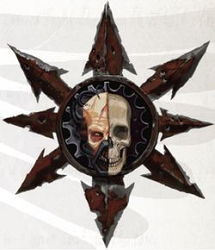
\includegraphics[width=\figwidth]{pics/11/42.png}
	\end{center}
\end{wrapfigure}
A quick  inspection of the system turned up the missing station farther back in its orbit of the local star than it should have been. 
In fact, a quick scan revealed that it wasn't in an orbit at all. 
It was moving in a nice straight line, right down the gravity well. 
The captain estimated it had passed the the point of no-return about four hours ago, and would start burning in around thirty. 
He refused to speculate on what sort of weapon or magic could just cancel an entire station's orbital velocity.

As for the ships, our initial instinct to go help the Imperial vessel was quelled when by the Captain. 
He reminded everyone that the only way the Occurrence Border would win a naval engagement was if the other ship spontaneously exploded before it fired its first broadside. 
If it exploded afterwards the fight would probably be a draw.

Furthermore, the ship was looking less and less like it needed our help the longer we looked at it. 
It was definitely a lot bigger than its opponent and was throwing out a staggering amount of firepower. 
Sure it seemed to be missing the smaller ship with every shot, but nothing the xenos was throwing out made it past their void shields. 
Also it was squawking stuff like *1010011010 FOR CHAOS 1010011010* across all vox channels and the Astropath refused to tell anyone what he was hearing. 
The tech-priest on duty on the bridge had immediately declared them to be Hereteks then had left his post to go talk to the other cogboys. 
No one bothered to stop him.

It was really looking like our best option was to just jump right back out of the system and head somewhere less creepy, that's certainly what the Captain recommended anyway. 
Except there was the tempting little matter of the station. 
It was the only thing in the system those ships could possibly be fighting over, and neither was in a position to stop us from taking a quick look…

It was a stupid, stupid idea and it's a miracle we survived.

\begin{wrapfigure}{O}{\figwidth}
	\begin{center}
		
\includegraphics[width=\figwidth]{pics/11/43.png}
	\end{center}
\end{wrapfigure}
The Captain had stubbornly refused to get any closer to either the station or the fighting ships than necessary. 
The Occurrence Border was positioned at nearly the maximum distance from the station its shuttles could travel and sat there with its engines and warp-drive spun up. 
In the Captains words, "If anyone even looks at me funny, I'm leaving all you stupid bastards to die."


With those encouraging words ringing in our ears everyone boarded their shuttles and went to see what was so special about the Way Station Alumentum Octavus. 
It says something about how distracted everyone was that we were cruising for about a quarter of an hour before we realized Jim was the one flying and Hannah was the co-pilot. 
The reunion was sort of spoiled by the little note taped to the cockpit door saying "The shuttle is monitored, talk and move as little as possible, wait for us to give the word."

After long and awkward wait Jim finally came back and announced that he'd looped something or other and we could talk. 
Hannah refused to leave the cockpit, even though we promised Tink wouldn't do anything weird. 
Aimy opened the conversation with a polite "What the hell is going on here you metal bastard?" but relented when Sarge vouched for Jim as the broest of cogbros.

The explanation that followed was quick, obviously well rehearsed, and fairly terrifying. 
The gist of it was that the ship's tech-priests weren't just ansty, they were on the edge of mutiny. 


\begin{wrapfigure}{O}{\figwidth}
	\begin{center}
		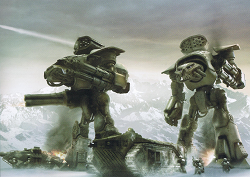
\includegraphics[width=\figwidth]{pics/11/44.png}
	\end{center}
\end{wrapfigure}
Jim hadn't seen the actual data they'd pulled out of the Magos, but whatever this piece of archeotech was, it had practically driven his seniors to a schism. 
Some of the cogboys wanted the tech destroyed, others wanted it locked away, and a few wanted to study it. 
The only thing preventing an immediate free-for-all was the fact that the thing wasn't here, and that the Magos had reported it to someone named Juris. 
The senior tech-priests had eventually agreed to wait for Juris to decide and abide by his decision. 
Unless, that is, it looked like the archeotech might fall into someone else's hands. 
Like say, the Inquisition's.

Less holy men, such as us or Jim, might see the ship's senior tech-priests as arrogant, socially stunted, and quite possibly insane, but they were NOT stupid. 
They knew we'd keep chasing the archeotech and would allow us to continue, for now, but were monitoring all the teams' shuttles and comms. 
If any of us found information relating to the archeotech or its location we'd be given a single chance to turn it over. 
If we refused, Jim and the tech-priests piloting the other shuttles had orders to cut our comms and return to the ship. 
Leaving all three teams to cook on the falling station. 
In his words, "The Magos Juris must decide this matter, anything else would result in a schism. 
When the Mechanicus schisms, titans walk and worlds burn. 
My superiors will see you all dead before they allow that."  

After everyone had digested this speech for a while Nubby put on his weaseliest smile and asked Jim if he'd really do that to his old pals. 
The flat look he got back from the enginseer was incredibly worrying, especially coupled with how Jim turned around and went back into the cockpit without saying anything else.

So anyway that's why, when we finally reached the station, our team decided to stay in the shuttle while the others went on ahead. 
They could probably handle anything in there without us.

\begin{wrapfigure}{O}{\figwidth}
	\begin{center}
		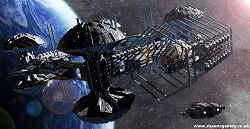
\includegraphics[width=\figwidth]{pics/11/45.png}
	\end{center}
\end{wrapfigure}
Sarge loudly announced to the other teams that he intended to do visual inspection of the station, y'know for space... 
stuff. 
The other Interrogators agreed it was a good idea, but none of us thought of it as anything more than an excuse not to get marooned on a rapidly falling chunk of metal by crazy cogboys. 
So it was quite a surprise when we cleared a corner and saw the Heretek shuttle already docked to the station.

We managed to call in the sighting just in time to keep the other teams from blundering into a bunch of heavily armed servitors and a tentically tech-priest. 
According to Battleaxe and Sword-guy the heretek seemed to be searching for something, stopping and doing creepy stuff to every cogitator or comm terminal he encountered. 
They decided that following the search party and seeing what it turned up was the best use of their time, and switched their teams to stealth mode. 
We wished them luck and continued our inspection.

Now this is where some less imaginative people would've blown up the docked shuttle, but we were suspicious bastards. 
Sure enough a little more searching turned up nearly a dozen more shuttles, all of them heavily armed but dormant for now. 
In our professional opinions twelve to three wasn't good odds, even without factoring in how much better armed they were than us; 
so Sarge decided to let sleeping shuttles lie and called in a warning to the ground teams, advising them not to engage. 
Battleaxe interrupted and asked him to repeat the message, it was hard to hear over all the shooting.

\begin{wrapfigure}{O}{\figwidth}
	\begin{center}
		
\includegraphics[width=\figwidth]{pics/11/46.png}
	\end{center}
\end{wrapfigure}
Luckily Sarge's facepalm turned out to be premature. 
Neither ground team was actually involved in the battle, they were just watching as some third party shot seven types of hell out of the patrol. 
The question of who the Hereteks were fighting was answered by the sight of a familiar lascannon beam stabbing out of the station hull a short distance away. 
Aimy summed up everyone's opinion of this development with an incredible streak of swearing.
 
Different people are curious about different things. 
Sword-guy was wondering what sort of convoluted plot the Eldar were running. 
Battleaxe was curious about what the Heretek was looking for in the cogitators. 
Our team didn't worry about that sort of complex bullshit; 
we just wanted to know how the Eldar had gotten onto the station, because we sure as hell didn't see any other shuttles out here.
 
Thanks to the adepts we all knew the pointy-eared bastards liked to use fancy hidden teleporting web dealies to get around, but that's not the sort of thing you find tucked into the corner of a human way station. 
Either their teleporters had range from where their ship was duking it out with the hereteks', which Jim claimed was incredibly unlikely, or someone was trying to be sneaky. 
Guardsmen don't like it when other people are sneaky, it typically ends with us getting shot in the back, so we decided to take a harder look at the station.
 
Since we didn't want to alert anyone to our presence out here, our moderately untrustworthy pilots did what they called a Passive Scan. 
We understood this to be the equivalent of looking real hard at something, but not going so far as to throw a rock at it to check for mines. 
Unfortunately, while it didn't blow our cover, it also didn't turn up anything. 
Sarge was debating ordering some figurative rock-throwing, when Tink announced that it was time to use some real scanners built by real scientists.

\begin{wrapfigure}{O}{\figwidth}
	\begin{center}
		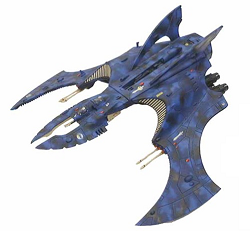
\includegraphics[width=\figwidth]{pics/11/47.png}
	\end{center}
\end{wrapfigure}
Jim hastily leaned out and tapped his "You are being monitored" sign before Tink finished pulling off Spot's skulls. 
There was an awkward sort of pantomimed argument, in which Jim managed to convey that he couldn't turn the cameras off again and Tink managed to convey that Jim was a colossal metal asshole. 
In the end Tink wound up putting on his void helmet and stepping out the lock with his drone before pulling off its disguise.
 
Since no one had anything better to do, we all clustered around the little airlock window and tried to watch over Tink's shoulder. 
It wasn't very interesting, all we could see was him poking at his xenos dataslate and muttering to himself. 
The real action was happening down below us, where the drone engaged its stealth field and started taking some very close looks at the station and shuttles. 
Whether it was due to Tink having a bit of experience looking for Eldar with his drone, or pure dumb luck, or because Tau drone tech was really just that good, he found a shuttle that was not like the others in just under five minutes. 
This did not please the Jim, who had to endure Tink making faces at him through the cockpit window as he relayed the drone's data.
 
What appeared to be a fairly standard, if gruesomely decorated, Imperial-style shuttle to our eyes, looked like a bat winged xenos craft to Spot the Wonder Drone. 
It had sharp, forward swept wings with odd chunks missing and these weird mandible-looking wings under the cockpit, but that wasn’t what really caught our attention. 
What really caught our attention was the two massive lascannons slung under it, this thing didn’t just have our shuttle’s little wing turrets outclassed, it had us completely out-schooled. 
Tink very carefully parked his drone above the xenos shuttle, and a quick debate over what to do about it was held.
 
It says something about how shaken we were by Jim’s little warning that we went with Nubby’s idea.

\begin{wrapfigure}{O}{\figwidth}
	\begin{center}
		
\includegraphics[width=\figwidth]{pics/11/48.png}
	\end{center}
\end{wrapfigure}
So no shit, there we were, hovering over a camouflaged xenos attack shuttle carrying more firepower than any three of our birds, and instead of running away or trying to destroy it before it realized we were there, we were trying to figure out how to steal it. 
The long warp voyage out to this backwater sector must have rotted our brains.
 
Quite aside from how stupidly dangerous an idea this was, it had absolutely nothing to do with why we’d come out here in the first place. 
In the station below us the other two teams had just engaged the Heretek forces in an effort to take a captive and figure out why they were here. 
In space above us two incredibly dangerous ships were locked in a brutal dog-fight while our own, completely combat-incapable, ship nervously watched from the sidelines. 
Somewhere across the immaterium an unknown archeotech device was cutting a swathe of destruction towards Imperial space. 
And yet, our primary concern was nicking this fancy looking xenos shuttle. 
Possibly while its owners were busy shooting up our companions. 
Truly we were the pinnacle of Inquisitorial professionalism.
 
It really wasn’t our fault though; 
the tech-priests were obviously to blame. 
If they hadn’t been plotting to maroon us in space, we wouldn’t have felt nearly so motivated to acquire an alternate means of transportation. 
When you combine that sort of threat with the opportunity offered by an incredibly valuable unattended vehicle, heretical xenotech though it may be, it’s entirely unreasonable to expect a poor guardsman to resist temptation.
 
Secure in the knowledge that our behavior was completely and totally justifiable, we prepped for our breaching tools and formed up in our shuttle’s airlock.

\begin{wrapfigure}{O}{\figwidth}
	\begin{center}
		
\includegraphics[width=\figwidth]{pics/11/49.png}
	\end{center}
\end{wrapfigure}
Twitch provided some cutting charges, which were carefully placed using the drone’s little servo arm. 
When everything was in place Jim, who’d eventually stopped trying to convince us to do something saner, flew us as close as he could without alarming any hostile shuttles. 
A trio of his little skulls were deployed and leashed like sled dogs, then he departed and us drifting in space above the holographically disguised shuttle. 
All things considered, it was a very good thing that Twitch was up to date on his meds and Fumbles wasn’t feeling particularly nervous.
 
The skulls hauled us across the gap as, just outside of our line of sight, the charges went off and the shuttle’s bay depressurized. 
As the last breath of air leaked out our five man, one woman team zipped in. 
We crossed into the grav field and landed inside the shuttle with weapons ready, just like the trained professionals we supposedly were. 
Well, at least five of us did. 
Whether it was due to her injured hand or because she wasn’t used to performing these sorts of shenanigans, Aimy missed her mark and wound of caroming off the hull. 
Everyone turned to watch as she spun off into space, swearing a blue streak as the skulls raced out to catch her. 
All of us were so distracted that we were nearly pushed out after her when a gust of wind suddenly hit us in the back.
 
Our squad turned around expecting to see, then shoot, some effeminate xenos. 
Instead, a pair of big scarecrow-lookin things with fish-shaped heads were standing there staring at us. 
At least we thought they were staring at us, the damned things didn’t have eyes. 
Their weapons were certainly pointed our way though, which was what really mattered.

\begin{wrapfigure}{O}{\figwidth}
	\begin{center}
		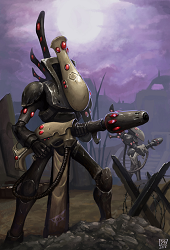
\includegraphics[width=\figwidth]{pics/11/50.png}
	\end{center}
\end{wrapfigure}
Fighting in a vacuum is odd: 
nothing sounds right. 
You can feel and sort of hear your weapons firing through your arms, but the shots don’t make a sound. 
It’s amazing how much you rely on little audio cues in a battle, it was hard as hell to tell how many shots we were firing and even harder to tell if they were hitting. 
Oddly, it was almost as if we’d lost exactly ten percent of our ballistics skills due to the unfamiliar terrain. 
We coped though, and poured a torrent of las and plasma fire into the two hostiles.
 
Surprisingly, the fish-headed xenos didn’t seem too bothered by our barrage. 
They just soaked our fire and slowly tracked their weapons onto us, then everything went funny. 
Not ha-ha funny, rather “Whoa I can taste the color purple with my ears” funny. 
As the feeling washed over us we scattered, and a pair of large orbs appeared. 


One orb formed right between Twitch and Sarge, while the other appeared above the now-prone form of Nubby. 
For a split second we could see something beyond understanding, but not horror, in the spheres. 
Then, with a pop that we could somehow hear through the vacuum, the orbs disappeared and took two perfectly circular chunks of bulkhead with them. 
We all just stood there and stared for a second, then Fumbles started screaming.

None of us had liked what we'd seen when the xenos had fired their weapons, whatever those things did looked a lot worse than just getting shot, but Fumbles had a stronger reaction than the rest of us. 
The little psyker's screaming ratcheted up to a shriek then kept going until it started bouncing around inside our heads.

Now there are several relatively normal things that are a bad idea to do in a void suit. 
Vomiting traditionally heads this list, followed by crying, sneezing, and a few other things depending on whether your model has waste disposal systems. 
Anyway, if someone ever revises the list, using a psychic shriek should probably be added somewhere near the top.

\begin{wrapfigure}{O}{\figwidth}
	\begin{center}
		\includegraphics[width=\figwidth]{pics/11/51.png}
	\end{center}
\end{wrapfigure}
Now, not being a psyker, I can't properly say whether it was a matter of the shout building up inside his helmet until something gave, or if it just punched through his faceplate on the way out towards its target. 
Either way though, we all felt a wave of panic roll over us as the shriek was cut off by what sounded like a burst of wind. 
A helmet's worth of air and a hail of plastic slammed into the two xenos monstrosities along with the psychic attack, where their combined force did exactly jack shit.

Fumbles landed on his ass, frantically clawing at his ruined helmet and radiating pants-wetting terror to the entire squad. 
Unlike our past experienced with the psyker's aura, this wasn't distracting, annoying, or disturbing: 
this was incapacitating. 
By all rights we should have died there, stumbling around in an attempt to escape a source-less fear, but two things saved us. 


The first thing was Twitch, who shrugged off the aura of fear like it was nothing. 
He sprinted across the room to Fumbles, pulling off his explosives-filled pack on the way. 
He jammed the bag over the psyker's head and pulled its drawstrings, causing the bag to inflate like an incredibly dangerous balloon. 
The aura of terror reduced in intensity as Fumbles' inability to draw a breath was replaced by claustrophobic darkness and the fact that someone was partially strangling him.

The second thing was that the fish-headed xenos were some sort of retarded. 
One of them fired a shot at Twitch as the trooper sprinted across the bay and missed by a scarily small margin. 
The other casually walked up the open hole in the bay and just sort of vacantly stared out of it. 
It didn't stop to shoot anyone on the way, or even try to step on Nubby who was lying half a meter from where it stopped. 
It was definitely one of the more bizarre thing we'd seen on a battlefield, or it would've been if we'd been in any condition to see anything.

\begin{wrapfigure}{O}{\figwidth}
	\begin{center}
		\includegraphics[width=\figwidth]{pics/11/52.png}
	\end{center}
\end{wrapfigure}
As the aura faded and we acclimated to the unusual feeling of someone else's terror raging through our minds, everyone got to their feet. 
We were greeted by the sight of one xenos reading his insanity-orb cannon for another shot, and the other spacing out at the edge of the hole we'd entered through. 
This is where your normal group of heroic badasses would've opened fire in an effort to kill the xenos before they could fire again. 
We didn't even try that.

See, our attacks, plasma and hot-shot lasgun alike, hadn't so much as phased these assholes; 
it was time to try something new. 
Sarge shouted his orders and threw himself at the xenos' cannon, grabbing onto it like a big, disgruntled monkey hanging from a branch. 
To Sarge's dismay, the fish-head turned out to be more than strong enough to hold up both him and the weapon. 
Luckily, the way Sarge was flailing around completely spoiled the xenos aim, and the next hell orb appeared in the middle of the bay's floor.

While Sarge kept his target off our backs, the rest of us turned to the one near the hole. 
Tink and Twitch stepped backwards, lowered their heads, and charged straight at the xenos' back. 
Down on the floor Nubby hastily crawled towards the hostile, then flipped onto his back. 
At this point the fish-head seemed to remember that it was in the middle of a battle and started to turn to face us, he wasn't fast enough though. 
Two charging guardsmen hit the xenos in the side at the same moment as a pair of augmetic legs launched upwards.

As body-checks went, they weren't the best: 
both soldiers were on the wiry side and the best word to describe the xenos' size and weight is Hulking. 
Combined with the lifting force of Nubby's legs though, it was just enough. 
In a sort of slow-motion ballet the fish-head tumbled forwards, right out of the hole we'd blasted into the bay's wall.

\begin{wrapfigure}{O}{\figwidth}
	\begin{center}
		\includegraphics[width=\figwidth]{pics/11/53.png}
	\end{center}
\end{wrapfigure}
Aimy was being hauled back towards the shuttle by Jim's skulls and Spot, who she was riding like some sort of demented horse. 
As she neared the hole something big and rather confused looking launched out of it, causing her to swear and nearly fall off her mount. 
After she regained her composure she watched as the... 
thing tumbled into the void, slowly spinning at it drifted away. 
When it didn't do anything she dismissed it as "not her problem" and raised her new rifle as the shuttle's interior finally came into view

Back inside the bay, the xenos had gotten tired of Sarge dangling off its weapon. 
It grabbed one of the struggling noncom's arms in a dinner-plate sized hand, and inexorably pried him of its weapon. 
Sarge found himself suspended in the air, or vacuum as it were, facing away from the angry xenos. 
He flailed as hard as he could in an attempt to break its grip and failed miserably. 
Sarge then grabbed his slung lasgun and tried to fire it over his shoulder, it was wrenched from his hand before he got more than a single burst off. 
Finally in desperation, he reached for his grenades, which were pretty high on the list of stupid weapons to use in a vacuum. 
Perhaps luckily, he wasn't able to grab one before his free arm was grabbed by the xenos' other hand. 
It raised him in the air then slowly, inexorably began to spread its arms, and by extension Sarge's, apart.

The first thing Aimy saw as she rose over the edge of the hole was Fumbles, sitting there and clawing at the backpack full of high-explosives tied over his head. 
This was odd, but not an immediate problem. 
The second thing, or things, were three of her squadmates running around like idiots and screaming about not being able to get a clear shot. 
The third thing was her new boss being pulled apart like a wishbone by a three meter tall xenos. 
Aimy sighted her rifle, waited a beat for Sarge's legs to swing out of the way, then put a burst of plasma right through the monstrosity's shoulder.

\begin{wrapfigure}{O}{\figwidth}
	\begin{center}
		\includegraphics[width=\figwidth]{pics/11/54.png}
	\end{center}
\end{wrapfigure}
In a perfect universe the fish-head's arm would've fallen off, then Sarge would've beat it around the head and neck with its own severed limb. 
Unfortunately in our reality the arm just went limp while the hand still retained its vice-like grip on Sarge. 
Also both of Sarge's shoulders were dislocated and he was too busy screaming to beat anyone around the anything. 
We tried not to let our disappointment show as Sarge merely flopped to the side and left us a clear shot at the xenos.

Three hot-shot lasguns, a plasma gun, and a pulse rifle poured precision fire into the xenos' thin middle-section. 
The combined weight of fire did what our earlier barrages couldn't, and with a soundless snap, the bastard collapsed in two separate pieces. 
Sarge swore loudly as he landed and informed everyone that the xenos' grip was not getting any looser.

Since the fish-head seemed rather hard to kill, most things lose their spunk after being cut in half y'know, everyone stepped forward and concentrated their fire on its shoulders. 
That finally did the trick and we pulled Sarge free, it took a while to pry the severed arms off of his wrists though, talk about a death-grip

We all stood there, contemplating our success and wondering what to do about Sarge's shoulders, when Fumbles finally caught our attention. 
His comm wasn't functional and we couldn't hear him, but he managed to send a rough psychic image out. 
He was wondering if the fight was over and we could go somewhere with air now. 
The bag was nice and all, but he was pretty sure at least one of the mines in there was armed. 


Twitch winced then he and Tink got to work on the door that the two fish-heads had come through. 
They had to push the xenos' severed torso out of the way to get access; 
it didn't do anything when Tink kicked it, but it somehow managed to glare reproachfully despite not having eyes, or any real face for that matter.

\begin{wrapfigure}{O}{\figwidth}
	\begin{center}
		\includegraphics[width=\figwidth]{pics/11/55.png}
	\end{center}
\end{wrapfigure}
While the more technical side of the team got the door open Jim's medi-skull floated in and took a look at Sarge. 
It sort of poked around in a confused manner, probably trying to figure out how to get at Sarge's shoulders. 
After a while its little machine-spirit must have reached a decision, because it deployed a syringe and tried to jab Sarge with it. 
The puncture-proof voidsuit turned out to be stronger than the skull expected: 
after a bit of straining it broke the needle and whacked into Sarge's shoulder, triggering an impressive amount of cursing. 
The medi-skull got even more agitated at this failure and deployed its little circular saw, the one we'd last seen it use to decapitate the Magos.

None of us really knew if it had decided to harvest Sarge's head, or just wanted to cut through his void suit,while he was in a vacuum so it could deliver its painkiller shot. 
Either way, Nubby and Aimy fended the skull off with the butts of their weapons until the door was finally opened. 
Jim was very apologetic about the whole thing, but we still didn't let the skull follow us into the pressurized section of the shuttle.

Once the door was closed and Twitch had carefully removed the bag full of explosives from Fumbles head, we looked around our new shuttle. 
The room where we'd fought the fish-heads had just been a moderately roomy troop compartment, nothing interesting in there; 
this room was definitely some sort of command center. 
It wasn't filled with vox units, cogitators, and random uninsulated wires like an Imperial command center, but the holo-thingy displaying a map of the station in the middle of the room was a dead giveaway.

\begin{wrapfigure}{O}{\figwidth}
	\begin{center}
		\includegraphics[width=\figwidth]{pics/11/56.png}
	\end{center}
\end{wrapfigure}
Despite its tasteful decor and abundant supply of air, the command room made us uneasy. 
It had a short hallway leading to the shuttle's cockpit, but none of us saw any hatches connected to the station. 
In fact the only exit we'd seen was the one on the rear, and it hadn't been connected to anything. 
The question of how the xenos had gotten aboard the station, and which direction they'd be coming from if they tried to take their shuttle back, hung in the air like a wet fart in a tank: 
hard to ignore and holding the potential to become a serious problem.

From the elegant, but rather uncomfortable, chair he'd found near the map, Sarge reminded everyone about how the xenos were supposed to use teleporting webs to get around. 
A brief search of the shuttle didn't turn up anything that looked like a teleportarium or was particularly web-shaped, the closest we got was a xenos rune that looked sort of like a spider. 
Twitch put a mine on it, just to be safe, then put a mine on everything else, just to be safer. 
None of us stopped him, it was really the only defensive option we could think of.

While Twitch saw to the perimeter, Tink got to work on figuring out how to fly our new piece of loot, Aimy checked in with the other teams, and Nubby called Doc for some medical advice. 
Sarge later complained bitterly about how many tries it'd taken to relocated his shoulders, but neither Nubby nor Fumbles had any medical training and there was a lot of distortion on the comm channel. 
Anyway the way he kept yelling was very distracting and the second one only took two tries, so all his whining wasn't really justified.
\begin{wrapfigure}{O}{\figwidth}
	\begin{center}
		\includegraphics[width=\figwidth]{pics/11/57.png}
	\end{center}
\end{wrapfigure}
After the little medical procedure was finished a quick council of war was held. 
Aimy reported that the other teams were just killing a lot of servitors, not making any real progress towards finding useful intel. 
Jim followed that up with a report that the tech-priests hadn't given any new orders, but claimed they were very interested in our shuttle. 


Based on all that, Sarge's vague plan was for us to call off the station part of the mission before anyone did something crazy and fly the Eldar shuttle back to the Occurrence Border. 
From there the adepts, and possibly the cogboys, could search it for clues or whatever. 
The only real problem with this plan was that compared to Imperial, or Tau systems for that matter, Eldar tech was almost impossible to understand. 
Tink was working hard, and kept claiming that he'd nearly figured it out, but so far he'd only managed to turn the lights on and off.

While Tink tinkered and occasionally asked for advice from Jim and Ol' Bill, the rest of us kept busy. 
Aimy watched the perimeter with Twitch, Sarge poked at the holo-map, and Nubby and Fumbles were assigned prisoner duty, prisoner in this case meaning the severed xenos toso. 
They taped the thing to the wall and, at Twitches request, drew a face on its blank head so it didn't look so creepy. 
At Nubby's urging, Fumbles was adding some embellishments to their artwork, when a section of wall slid outwards and a tall, lithe, and familiar-looking xenos appeared out of thin air.

The Eldar Warlock scanned the room then began to say something. 
He was immediately interrupted by Twitch shouting that a hostile had breached the perimeter and raising his lasgun. 
The xenos tried to resume speaking, only to be interrupted again as Twitch asked for permission to fire. 
Sarge, who'd nodded off, jerked awake just in time to hear the frustrated Eldar snap: 


\greentext{>Foolish mon-keigh, you can't shoot me I'm a h-}


Then Twitch got tired of waiting and opened up on full auto.
\begin{wrapfigure}{O}{\figwidth}
	\begin{center}
		\includegraphics[width=\figwidth]{pics/11/58.png}
	\end{center}
\end{wrapfigure}
There are times when an Inquisitorial agent, military commander, or Imperial diplomat will negotiate with one of the hated xenos and discover that they really aren't all that bad. 
Then they wind up working together to fight some common foe, and a sort of polite, but distant, working-relationship based on mutual respect is formed. 
This was not one of those times.

It took the Warlock about five tries to finish saying "hologram", Twitch kept shooting him every time he started talking. 
When the demolitions trooper finally ran out of ammo the incredibly frustrated Eldar exploded into a lecture on how holograms work and why it was pointless to shoot them. 
He was interrupted halfway through as Nubby shot him, turned towards Sarge, and reported that "The Xenos 'pears ta be some sort of 'ologram, I don fink we can shoot 'im". 
The Eldar swore in its fancy language and asked Sarge to control his "ape creature," whereupon Twitch finished reloading and shot him again while Nubby loudly told Sarge that the xenos was getting pissy. 
Things only went downhill from there.

The warlock was an arrogant bastard. 
He tried to order us around, but none of us had even the slightest intention of "returning to our wretched vessel" or "leaving matters beyond our comprehension to our betters." The diplomatic breakdown was total: 
on our side of the table Aimy had a serious axe to grind, Nubby was just Nubby, Sarge's shoulders hurt like a bitch, and everyone else just didn't give a shit. 
As for the Warlock, he loudly declared us to be idiot children playing with deadly weapons, both personally and as a race.

\begin{wrapfigure}{O}{\figwidth}
	\begin{center}
		\includegraphics[width=\figwidth]{pics/11/59.png}
	\end{center}
\end{wrapfigure}
The Eldar had probably intended to either use his moral superiority to get us to leave his ship, or cut some sort of deal with us. 
The problem was that he kept getting bogged down in pointless arguments, petty insults, and fits of frustrated anger. 
Everyone, even Fumbles, was doing something that might as well have been scientifically designed to outrage the prissy xenos.

To start with, Tink didn't even try to hide the fact that he was stealing the Eldar's shuttle, and occasionally asked him what a specific button did. 
Aimy only spoke when she'd thought of something particularly scathing to say and while Twitch eventually stopped shooting the hologram, he'd occasionally interrupt the Warlock to insert his own rather unique theories into the conversation. 
Fumbles, who was admittedly acting on Nubby's orders, doodled on the captive fish-headed xenos. 
This caused a surprising amount of anger in the Warlock, despite how good the mustache and monocle he drew looked. 
All that was relatively minor compared to Nubby and Sarge though.

Nubby, for reasons beyond all logic, had appointed himself as the Warlock's translator. 
He shouted down or shot the holographic xenos at the end of almost every sentence, then relayed his personal interpretation to Sarge. 
Our fearless leader took an evil delight in how much this annoyed the Eldar, and started only responding to Nubby's translations. 
It was childish, antagonistic, incredibly unprofessional, and all according to a plan so devious that none of us even realized we were part of it. 
Well, at least Sarge claimed it was his plan afterwards, and no one was in any position to argue with the results.

\begin{wrapfigure}{O}{\figwidth}
	\begin{center}
		\includegraphics[width=\figwidth]{pics/11/60.png}
	\end{center}
\end{wrapfigure}
In his most cunning of minds, Sarge figured that the Warlock had us incredibly outclassed when it came to diplomacy. 
The only person on our team that stood even a chance a of holding their own was the old diplomat adept back on the ship, but with the cogboys monitoring the comms, bringing him in was out of the question. 
Therefore, the only way we could possibly come out ahead in a negotiation with an Eldar, who probably had hundreds of years of experience talking circles around Inquisitors and the like, was to drag him down to our level. 


Now, the brilliance of Sarge's plan didn't end there. 
In addition to keeping the Eldar off balance, the behavior of the more… eccentric members of our squad acted as a time-buying distraction for both Tink and the other teams. 
Every second the Warlock spent screaming at us in incoherent rage, was a second where he wasn't leading an attack on our shuttle or sniping anyone in the station. 
Admittedly, neither group was actually accomplishing anything useful with that time, Tink had found thirteen different controls for the shuttle's lights and last we'd heard the other teams they were still killing endless waves of servitors, but they did have it.

The incredibly uncivil discussion eventually rolled around to how stupid humanity's fascination with archeotech was. 
Our race's suicidal persistence in trying to keep the current piece from its owners was going to wind up gutting the entire sector's ability to fight off the next wave of tyranids. 
On top of that, if we somehow managed to keep it we'd inevitably wind up destroying ourselves with it. 
Any sane race would've let the Necrons have it, or at least dropped it on some Ork or Tyranid world that no one would miss.

Sarge perked up at this piece of actual useful information. 
Then, when Nubby suggested his cunning new idea to drop the archeotech on some Ork or Tyranid world that no one would miss, Sarge agreed that it was a good one. 
The Eldar paused mid-rant to boggle.

\begin{wrapfigure}{O}{\figwidth}
	\begin{center}
		\includegraphics[width=\figwidth]{pics/11/61.png}
	\end{center}
\end{wrapfigure}
The incredulous Warlock asked if we were serious. 
Sensing that the time was right, Sarge told Nubby to shut up, and promised that he was super serious. 
We didn't want to use the archeotech, we didn't want to study the archeotech, and we certainly didn't want to fight Necrons, Emperor help us, for the archeotech. 
As far as any of us were concerned, the metal bastards could have the thing.

The Eldar sputtered, then asked about fifteen different questions, most of which he answered himself. 
We were obviously too stupid to lie and we must have already known what the archeotech was, otherwise how'd we know to come to this system? 
Furthermore, despite our appearance and behavior, we were obviously the ones in charge of the mission. 
After all, our team was the one in his shuttle as opposed to fighting servitors on the station. 
No one correct these assumptions.

The only real question the Eldar had for us was why we wanted the archeotech destroyed. 
According to him, the five other Inquisitors and Magi he'd encountered, then killed, had all lusted after the device like it was mankind's salvation. 
Sarge nonchalantly suggested that we were just smarter than them. 
The Warlock shot a pointed look at Nubby, who had a finger jammed up to the second joint in one of his nostrils, then back to Sarge. 
Our fearless leader shrugged and adjusted that to "less ambitious than them."

\begin{wrapfigure}{O}{\figwidth}
	\begin{center}
		\includegraphics[width=\figwidth]{pics/11/62.png}
	\end{center}
\end{wrapfigure}
Before anyone else could say anything to push the Warlock back from confused to furious, Sarge made his move. 
He pointed out how we only wanted to prevent any more planets being wiped out. 
We agreed with the Eldar, the archeotech either needed to be destroyed, turned over to the Necrons, or sent out of Imperial space. 
So he should just tell us where it was going next and we'd handle the rest. 
There'd be no working together bullshit: 
we'd leave as soon as we had our directions, and he'd never have to talk to us again.

The Warlock started to say something, then stopped, then started again, then stopped again. 
Finally he let out very frustrated sigh and gave us directions to an Imperial world whose Governor had just purchased the archeotech. 
The Eldar then told us to get off his shuttle before he ordered his ship to disengage and let the hereteks have the system, data records and all. 
Sarge took a second to ponder this last part of the deal, and asked Tink how things were going.

From up in the cockpit Tink announced, for the twentieth time, that he'd figured out the controls and would be able to fly us away before anyone could stop us. 
He triumphantly pressed a few buttons, flipped a switch, and manually connected two wires. 
Once again, the shuttle completely failed to move and the lights flicked off then back on. 
Sarge told the Warlock he could have his shuttle back.

\begin{wrapfigure}{O}{\figwidth}
	\begin{center}
		\includegraphics[width=\figwidth]{pics/11/63.png}
	\end{center}
\end{wrapfigure}
Twitch packed up his toys, Fumbles was given a less dangerous pack to use as a helmet, Tink was forcefully pulled out of the cockpit, and Nubby was told to empty his pockets. 
While everyone else packed up Sarge and Aimy debated the whole tech-priest problem, it was eventually decided that there was no way to really hide the archeotech's location from them. 
Luckily, Aimy was able to suggest a way to keep the cogboys on our side for the time being.

Jim was called to pick us up, and over the monitored channel Sarge reported the location of the archeotech. 
He also warned everyone that a sizable Heretek fleet was being gathered to seize it before the mechanicus could confiscate it, so maybe we should try to get there and secure it first. 
It wasn't very subtle, but hey, neither were we, and the cogboys must've bought it, because everyone's shuttles picked them up without any arguing or ultimatums. 
Everyone was feeling pretty happy about how the mission had went as we left the Eldar shuttle. 
In a fit of goodwill Tink even pushed the fish-head's limbs into a neat pile and left a note saying which way second one had been drifting when we'd last seen it.

As Jim and Hannah flew us back to the Occurrence Border, we looked back at the station we'd never gotten around to boarding. 
It was looking rather ragged, its interior probably hadn't been designed to survive pitched fights involving anti-armor energy weaponry, and the star behind it had gotten noticeably larger. 
We congratulated ourselves on not being stupid enough to board that deathtrap, and watched the station shrink behind us. 
Right as it was getting too small to see anymore, there was a neat little firework display. 
We couldn't be sure, but the explosions seemed to match the locations of all the heretek shuttles. 
That probably explained what the Eldar had been up to.

\begin{wrapfigure}{O}{\figwidth}
	\begin{center}
		\includegraphics[width=\figwidth]{pics/11/64.png}
	\end{center}
\end{wrapfigure}
Our good moods lasted until Jim landed us in the Occurrence Border's main shuttlebay. 
We were the last team back and the bay was a madhouse full of rushing people and horrible screams. 
Doc and his girlfriend were running around with their medical team, from the look of it they had quite a few customers and Sarge detailed a few of us to lend a hand. 
Surprisingly, most of the screams weren't coming from Doc's patients. 
What had at first looked, and sounded, like a field surgery station turned out to be something weirder.

Half a dozen of the senior cogboys were clustered together in a far corner of the bay. 
As we watched a captive heretek was brought off of a shuttle by some servitors and dragged into the group of tech-priests. 
There were some very unsettling power-tool noises and a lot more screams, and Sarge asked Jim and Hannah what was going on. 
The two Enginseers whispered to each other for a while then said the tech-priests were checking the captives for… serial numbers. 
Apparently they could be used to determine which Cabal the hereteks had come from. 
From there the tech-priests would research past records of the sort of technology the hereteks had access to, giving us a major advantage when it came time to fight their fleet. 


Sarge pondered the fact that there wasn't actually any heretek fleet. 
He then weighed that against how the screams seemed to indicate that the cogboys didn't believe in little things like sedation, or killing people before dissecting them. 
In the end he decided that this was not his problem and he really needed a drink, or at least some painkillers for his shoulders. 
Better yet a drink and some painkillers and someone to take his void-suit off without him having to move his arms. 
In the end he had to settle for just the painkillers, everything else had to wait until after he'd talked with the Captain, adepts, other Interrogators, and whoever the tech-priests sent to vaguely threaten everyone.

\begin{wrapfigure}{O}{\figwidth}
	\begin{center}
		\includegraphics[width=\figwidth]{pics/11/65.png}
	\end{center}
\end{wrapfigure}
Sarge returned to our quarters hours later, looking like shit and still wearing his void-suit. 
Our first few tries to remove his suit resulted in a lot of yelling and Nubby getting punted across the room. 
In the end Tink wound up just cutting him out while Aimy held a bottle of liquor with a straw in it for him.

The gist of the situation was that the Eldar ship had disengaged and vanished after the heretek shuttles had been destroyed. 
The heretek ship hadn't tried to chase us or catch up with the falling station, instead it had  warped out shortly after the fight ended. 
The Captain couldn't be sure, but it didn't look like it was heading the same direction as us, and the scanners had been clear since we entered the warp ourselves.

We were headed towards the coordinates the Eldar had given us, which had turned out to be the planet with the shifty governor Sword-guy had wanted us to go to. 
Sarge said the other Interrogator had been rather bitter over the whole thing, mostly on account of how he'd been shot in the gut twice during the station fight. 
Battleaxe wasn't in great shape either, they'd shed a lot of blood fighting off the servitors and capturing two hereteks for interrogation. 
Tensions were rather high due to the way the tech-priests had seized those hard-won prisoners and vivisected them. 
The cogboys were not very apologetic for this, but at least they'd shared their info on this particular group hereteks with the rest of us. 
The adepts were chewing through it and would be putting together some combat plans and stuff like that during the trip.

The other info Sarge had relayed from the Warlock hadn't gone over well. 
To start with, everyone but the tech-priests had given Sarge grief for not getting the actual details of the archeotech from the Eldar. 
He'd very politely told them where they could shove their complaints, then moved on to the matter of who was probably purging planets. 


\begin{wrapfigure}{O}{\figwidth}
	\begin{center}
		\includegraphics[width=\figwidth]{pics/11/66.png}
	\end{center}
\end{wrapfigure}
The revelation that it was Necrons chasing the archeotech, or at least that the Eldar said it was the Necrons, had quieted everyone down. 
While it had been the smart bet in the pool ever since we'd learned this was all about a piece of archeotech, having it confirmed was fairly unpleasant. 
None of the other teams had fought them before, but between their training and the stories everyone had heard, they didn't need us to tell them that the Necrons were bad news.

The Captain had reiterated his suggestion that we go somewhere safe and request an entire fleet's worth of backup. 
Most of us thought that sounded like a great idea, unfortunately Sarge and the other Interrogators thought otherwise. 
They believed that if we got there fast enough we could do something to prevent Necrons from wiping out the planet and keep the heretek fleet, which Sarge now regretted making up, from getting the archeotech. 


Of course the exact details of what we'd do were still a bit fuzzy. 
The Interrogators' only good ideas were to either destroy the archeotech, or put it somewhere where the Necrons could take it without killing everyone. 
The tech-priests had informed everyone that both those options would result in their grisly deaths. 
The most they'd allow would be for us to set up a perimeter around the archeotech and plant a bomb which the ship's head tech-priest would build and hold the only detonator for. 
All the Interrogators, even Sarge, had wound up agreeing to this. 
The Captain had called them idiots and, since Sarge wasn't in any condition to hit us at the moment, we all agreed.

The one saving grace of the Interrogators' plan was that, being on the border and all, the planet we were heading towards had a fair sized PDF and SDF. 
Between that and the detailed intel we could provide, there was a slim chance we could hold off the Necrons until reinforcements arrived or the tech-priests stopping being assholes. 
Emphasis on slim.

\begin{wrapfigure}{O}{\figwidth}
	\begin{center}
		\includegraphics[width=\figwidth]{pics/11/67.png}
	\end{center}
\end{wrapfigure}
Once again we were stuck travelling through the warp and hoping like hell we'd arrive before everything went ploin shaped. 
At least this time we had a better idea of what was currently happening at our destination: 
the planet had a branch of the Telepathica and our astropath was able to keep tabs on their situation. 
The adepts and other teams spent a lot of time sending messages back and forth, looking for clues about where the archeotech was and all that. 
We didn't trouble ourselves with any of that, someone would tell if they found something important, for the time being we had other stuff to do.

Aside from the usual planning bullshit that Sarge had to put up with, we were able to dedicate our full efforts to some very important projects. 
Okay, well one important project, a less-important minor one, and a bit of "entrapaneering". 
The less-important one was replacing Sarge's lasgun. 
When the xenos, which the adepts had told us was called a Wraithguard not a fish-head, had disarmed him it'd bent his lasgun like a banana. 
Since fruit-shaped weapons tend not to work well and Aimy's pulse-rifle had performed so awesomely, Tink put all his effort into converting a Tau carbine for Sarge's use. 
Everyone else was moderately jealous.

The other side project was, of course, Nubby's continual quest not to lose quite a lot of money in the betting pool. 
Fumbles revealed to the rest of us that during our last bit of travel time they'd tracked down the only three people who'd bet on the Necrons, then… persuaded them to retract those bets. 
All that was left to do was convince the ship's quartermaster, who was the one actually holding the money and tracking the bets, to allow the withdrawal. 
Once that was done there'd be no winning bets, and the money would surely default back to everyone. 
We left Nubby to his little plot, which seemed to revolve around getting some incriminating pictures of the quartermaster. 
We'd be getting our money back too after all.
\begin{wrapfigure}{O}{\figwidth}
	\begin{center}
		\includegraphics[width=\figwidth]{pics/11/68.png}
	\end{center}
\end{wrapfigure}
So, aside from that little stuff, all of our effort was put into the big important project: 
Operation Screw Everyone Else Over Before They Screw Us. 
Now, this may sound like the default state we operated in, but this was a much more concerted effort than our usual paranoia and misanthropy. 
Our focus was almost entirely on two parties: 
the tech-priests and the Warlock. 
Now, it's obvious why we felt the need to plot against the cogboys with them acting nuttier than squirrel shit and all, but that Eldar part might need some explanation.

See, it is in the very nature of Eldar to dick honest, hard-working guardsmen over. 
They probably tell each other stories of great Eldar heroes who use their magical xenos powers for absolutely nothing but being a colossal dick. 
Based on this single concrete fact about his basic nature, we knew that the Warlock would A: 
Show up at the planet, B: 
Try and to use us to destroy the archeotech, C: 
Proceed to dick us over as hard as he possibly could the second we were no longer useful. 
The may be a lot to infer from a single piece of racism, but it was backed up by our personal experience with the Warlock. 
When we'd been talking with him over the holo-whatsit, we'd gotten the distinct impression that he didn't like us for some reason; 
that was a sure sign of a dickish personality.

Anyway, the project was mostly prep-work and the first step was securing allies. 
Jim and Hannah had been decent to us, but that whole thing about possibly following orders to leave us to die was bad and needed fixing. 
To that end, both Jim and Hannah were invited down to our quarters, then locked in and treated to a class on Ethics by our resident expert: 
Nubby.

\begin{wrapfigure}{O}{\figwidth}
	\begin{center}
		\includegraphics[width=\figwidth]{pics/11/69.png}
	\end{center}
\end{wrapfigure}
Don't laugh, this wasn't a class on any of those sissy "Do unto others as you would have them do unto you" Ethics. 
This was a class on Guardsmen Ethics, which tend to only go as far as "Do unto others," and Nubby knew those by heart. 
He and Doc, as what you might call the friendliest and most persuasive members of our little group, were assisted by the ever-loyal Fumbles in teaching Camaraderie 101 to Jim and Hannah.

The two junior tech-priests were educated in: 

\greentext{>Why it is Important to Stick With Your Mates}

\greentext{>When and When Not to Follow the Rules and Regs}

\greentext{>Why You Should Never Trust Anyone Over the Rank of Sergeant}

They also got a special bonus course on:
\greentext{>Why Killing Your Close Personal Friends Because a Crazy Priest Told You to is a Very Bad Thing}


By the end both enginseers were thinking like proper Guardsmen and gave us all the vital information we needed for the rest of our project. 
Specifically, how the tech-priests would probably monitor us, what sort of bomb they'd be giving us to plant, and where it and its detonator were being built. 
From there it was Twitch and Tink's show.

Twitch was far, far too excited about his part of the plan. 
Not because he got to blow up people who annoyed him, Sarge had vetoed mining the priests' quarters on account of how we wanted to still have a ship after the mission, but because he got to play with the biggest bomb he'd ever seen. 
Now, when I say biggest I don't mean it's size, I mean its yield. 
The first time Twitch made his way through the vents to where the priests were putting the bomb together, he'd wound up needing a new pair of pants. 
They were giving us a backpack nuke.

\begin{wrapfigure}{O}{\figwidth}
	\begin{center}
		\includegraphics[width=\figwidth]{pics/11/70.png}
	\end{center}
\end{wrapfigure}
It's been said, mostly by guardsmen, that the final step of becoming a full tech-priest involves having the common sense part of your brain pulled out and replaced with a little box of screws. 
In our opinion, the fact that they were giving us a nuclear weapon pretty much proved that.

Of course they thought that they'd be the ones controlling it. 
They probably snickered to each other about how frustrated and scared we'd be, not being able to set off the bomb after planting it and not knowing if they'd remotely detonate it while we were in the blast radius. 
Still though it was a titanically bad idea, I mean even ignoring how much trouble we were able to cause with conventional explosives, we had a demolitions expert and what could loosely be called a technical expert on our squad. 
The second we were out of their line of sight we were going to crack that puppy open and rewire the detonator.

So Tink and Twitch spent their time spying on the bomb's construction and planning how they'd rewire it and jam the cogboys' bugs. 
Meanwhile, the job of putting together a plan to screw over the Eldar fell to Aimy and Doc, largely because they were willing to do what the rest of us were not: 
sit through tedious lectures on xeno-psychology from the adepts. 


Unfortunately, we didn't know exactly what the Warlock had was going to do, only that dickishness would inevitably be involved. 
This meant that Doc and Aimy could only come up with sort of general plans, but they still did a very good job of it. 
A bunch of contingencies were prepared for, a few simple strategies were mapped out and practiced by our entire team, and Aimy came up with a rather nasty idea for forcing to Warlock to behave if we ever saw him in person. 
Doc quietly told the rest of us that he was glad not to be evil master-mind this time around, and recommended we never antagonize the markswoman.

\begin{wrapfigure}{O}{\figwidth}
	\begin{center}
		\includegraphics[width=\figwidth]{pics/11/71.png}
	\end{center}
\end{wrapfigure}
When we finally came out of warp at the border world we felt ready for anything. 
Unfortunately it turned out that the other teams and adepts weren't nearly as awesome as us. 
Not only had they failed to pin down the location of the archeotech for us, they'd also been unable to confirm that it was even in the system. 
Sure, a quarter of them had died fighting on the station, and half the survivors were still being tended to by Doc and his girl, AND they'd only been able to do their research via discrete astropathic questioning and a few out of date field reports. 
Still though, we'd expected better of them. 
I mean a little professionalism and work ethic isn't much to ask is it? 
It was going to be so damned embarrassing if turned out that the Eldar had been lying to us.

We sat on the ship for a few days, twiddling our thumbs and getting more and more worried while the other teams went down and made some discreet inquiries. 
Sarge and the adepts helped them out, but the rest of us pretty much stayed in orbit and waited for the word go. 
Luckily, from our perspective, they met with enough resistance from the local government and ad-mech priesthood to practically prove the archeotech was there somewhere. 


Probably the only reason that no one tried to kill our investigators was the constant stream of ships pouring into the system at our request for reinforcements. 
Most of them were little navigator-less armed merchantmen, but there were a few escort-class vessels, and the Captain said our odds in a naval battle were definitely looking up. 
Still though, from what we overheard, the locals were some seriously uncooperative people. 
No one would admit to anything, even when the Interrogators started flashing their junior-rosettes around. 
That changed abruptly when every astropath and navigator in the system reported a fleet approaching through the warp.

\begin{wrapfigure}{O}{\figwidth}
	\begin{center}
		\includegraphics[width=\figwidth]{pics/11/72.png}
	\end{center}
\end{wrapfigure}
While the incoming fleet was great for our investigation, it was also rather confusing. 
The only thing anyone knew for certain about how Necrons got their ships around was that they didn't use the warp. 
Of course everyone else said it was the Heretek fleet, but we knew better and spent a lot of time pondering what was actually coming. 


Honestly it got very annoying telling everyone it wouldn't be a Heretek fleet then not being able to say why. 
Sarge finally snapped during the final big meeting, and just told everyone he'd made the fleet up to keep the tech-priests in line. 
There was a lot of arguing and shouting after that, but luckily no mass servitor uprisings.

Of course about five minutes after he said that, a large group of what were unmistakably Heretek vessels came out of the warp and demanded the surrender of all technology within the system. 
Everyone was too busy for much recrimination, but the Captain did spare a few seconds to congratulate Sarge on being psychic.

With the arrival of the Heretek fleet everything started happening at once. 
Sword-guy, who was still too injured to help much in combat, transferred over to the largest friendly ship in system and started organizing the took overall command of fleet we'd been cobbling together. 
Armed with the intel provided by our ship's priests about the Hereteks' probable armament and strategy, he was confident that he could keep the hostile fleet away from the planet for at least a day or two. 
Down on the planet Battleaxe, who'd been leading the investigation, was approached by several local nobles who'd had a change of heart.

\begin{wrapfigure}{O}{\figwidth}
	\begin{center}
		\includegraphics[width=\figwidth]{pics/11/73.png}
	\end{center}
\end{wrapfigure}
The planet's nobles sold out their governor and put their forces at Battleaxe's command. 
The basic story they gave us was that the Planetary Governor had purchased the piece of archeotech and a team of scientists from a Rogue Trader. 
The device itself wasn't being used for anything, and they didn't actually know what it was, but the technology being reverse engineered from it was supposed to turn their little SDF fleet into the most powerful space force this side of Battlefleet Ultima. 
They were patriots see, it had all been for the good of their world, and by extension the Imperium.

The Governor had told them all that within five years they'd be completely secure against any Tau aggression or Tyranid splinter fleets. 
In ten their shipyards would be the envy of every forge-world. 
In twenty they'd personally control all space-shipping from there to the Damocles Gulf. 
And by the end of the century, the Administratum would need to make a whole new sector just to contain the worlds they'd use their fleet to colonize and take back from the Tau. 
Quite the statement, but every tech-priest and veteran voidsman they'd sent to look at thing had confirmed it. 


So they'd all signed on, even knowing that some xenos force was chasing the archeotech and would need to be fought off. 
They were confident in size of their defence forces, they said. 
All those other worlds that'd been wiped out were little undefended backwaters, they said. 
It was worth the gamble, they said. 
But now that they saw the size of the Heretek fleet and the Inquisition was at their door, they were singing a different tune.

\begin{wrapfigure}{O}{\figwidth}
	\begin{center}
		\includegraphics[width=\figwidth]{pics/11/74.png}
	\end{center}
\end{wrapfigure}
Up in our shuttle we were listening in to the whole spiel as we dropped towards the manufactorum they'd fingered. 
Everyone but Jim and Hannah, who were locked in the cockpit and keeping to themselves, speculated on just what sort of super-weapon they'd found. 
If it really was such a big game changer it'd be a shame to just blow it to little radioactive pieces.

We were still going to do it of course. 
Aside from the whole thing where it was heretical piece of archeotech with the potential to drive the mechanicus to schism, you can't carry a nuke all the way down to a planet and NOT set it off. 
It's just now allowed. 


Anyway, as we went to go blow up the archeotech, Battleaxe was organizing a coup. 
She and her half-strength team would handle capturing the Planetary Governor and securing a temporary government with the help of most of the Nobs' regiments. 
She wasn't hogging all the support troops though, a sizeable force had been stationed near the manufactorum where the archeotech was located, and she sent them to lend us a hand. 
Well, actually it was more a case of us lending them a hand, they had a lot less travel time than us and we saw nothing wrong with them handling most of the grunt work.

So our little eight man force came down outside the manufactorum after several hundred PDF yahoos had spent about an hour shooting the place all to hell. 
That may not have been quite as professional as leading some sort of high-precision strike force, but the important thing is that the place was clear and none of us had gotten shot in the process. 
Whole lotta PDF had though, the place was a mess. 
That's what happens when you're dumb enough to try to rush fortified positions. 
Poor dumb Guard wannabees.

\begin{wrapfigure}{O}{\figwidth}
	\begin{center}
		\includegraphics[width=\figwidth]{pics/11/75.png}
	\end{center}
\end{wrapfigure}
Per our orders the PDF had stayed out of the semi-secret basement where the archeotech was located. 
They'd just swept the upper building, which had been defended by a few of the Governor's men and as well as a surprisingly large number of servitors. 
The servitors worried us at first, since the Hereteks weren't supposed to be anywhere near close enough to shuttle or teleport a force down. 
Thankfully, when Jim and Hannah came over to take a look they said the servitors didn't have any recognizable Heretek markings. 
That was a load off our minds, and we followed some PDF General over to the basement entrance. 


Surprisingly, Jim and Hannah both tagged along instead of returning to their shuttle. 
Sarge weighed the pros and cons of having two cogboys around when we went to blow up some piece of really cool tech, then decided to trust them. 
The Enginseers fell in behind Twitch, who was lugging a rather heavy backpack containing a large metal metal cylinder with an unnecessary amount of ornamentation on its surface. 


The bomb did not have any exterior controls, readouts, or anything aside from what Jim told us were etchings of holy scenes and prayers written in binary. 
It looked like a drum for storing holy water more than anything, it was about the right size and weight. 
We'd had to scrounge a grav plate and clamp it to the bottom for anyone but Sarge to be able to carry the thing. 


Presumably the whole reason for the bomb's odd design was that there were no exposed controls for us to muck around with and no way to see inside. 
It should've stopped anyone who wasn't entirely suicidal from trying to go in and rewire its detonator, but Twitch had the thing cut open within ten minutes of our shuttle's departure. 
Now the nuke's top was held on with duct-tape, its remote control was hooked up to a novelty noise-maker, and the only way to set it off was using the detonator Sarge was carrying.

\begin{wrapfigure}{O}{\figwidth}
	\begin{center}
		\includegraphics[width=\figwidth]{pics/11/76.png}
	\end{center}
\end{wrapfigure}
After a rather unpleasant walk through the corpse-filled building we reached the entrance to the underground lab where the archeotech was stored. 
We stood around the intimidating entrance for a while, wondering just what sort of defenses were waiting down there, and if it would do any harm to send a few squads of PDF down first. 
Our little debate was interrupted by a call from the Captain, who warned us that the fleet engagement had started and that, inexplicably, all astropathic communication was being blocked. 
Jim blanched at hearing that second part, and told the rest of us that the hereteks didn't have a way to do that, the Necrons were here.

Confirmation arrived in the form of a few dozen green lighting storms outside the windows. 
They weren't violent enough to be an orbital bombardment and faded quickly, but they left behind some very ominous glowing clouds. 
Tink went over to a window and ratcheted up the zoom on his goggles, then went pale and recommended that we go blow up the archeotech RIGHT NOW. 
There wasn't time to fool around with sending scouts down there, and anyway the PDF would need all the men they had to fight off the millions of metal insects that'd just teleported into the atmosphere. 
We didn't need telling twice and practically sprinted into the basement, only stopping to advise the PDF general to conserve ammo and save his last round for himself.

Twitch and Fumbles went first to check for traps or ambushes. 
Sarge tried to take the nuke from Twitch before he took point, but the demolitions trooper flatly refused. 
He claimed the bomb was his now, and he'd be damned if anyone would take it from him. 
Anyway he said it wasn't getting in his way and it actually helped him concentrate; 
just carrying it made him feel all warm and fuzzy inside, he said. 
The rest of us thought that that sounded like it was leaking radiation, but didn't push the issue.

\begin{wrapfigure}{O}{\figwidth}
	\begin{center}
		\includegraphics[width=\figwidth]{pics/11/77.png}
	\end{center}
\end{wrapfigure}
Aside from a few traps which Twitch easily disarmed, the stairs down weren't defended by anyone. 
Either they'd all fought and died on the surface, or they'd fallen back the the big room at the bottom of the stairs. 
We all bet on the latter and formed up to breach the final door.

The charge went off, flashes were tossed, and we all rushed in with weapons raised. 
Then we all sheepishly walked down the empty hallway to what was was ACTUALLY the final door, and did all that again.

This time a hail of las fire poured at us as we scrambled to find cover in a very large room. 
Luckily, in addition to being very large, the room was littered with all sorts of conduits, machinery, and inexplicably chest-high walls. 
Through a combination of luck and skill we all managed to find something solid to hide behind and started trading fire with what looked to be five tech-priests.

Originally we'd had some vague plan that Tink would find where in the room the archeotech was and Twitch would plant the bomb while the rest of us held off the defenders, but that didn't turn out to be necessary. 
For one thing, it was easy to see where the archeotech was, a MASSIVE opaque shield took up the rear half of the room. 
For another, the tech-priests didn't need to be held off, they were pathetic. 
These guys weren't anything like the sort of mechanical combat-monstrosities we'd expected, they were just relatively normal tech-priests with las-pistols. 
They holed up behind some ineffective cover and we picked them off one by one while Jim and Hannah made a half-hearted attempt to negotiate their surrender.

There was just one of the tech-priests left, and we were arguing over whether to try and take him alive so he could deactivate the shield. 
Then we all heard a metal stomping sound and something that looked like a cross between a dreadnought, a necron, and a metal squid came around the edge of the shield.

\begin{wrapfigure}{O}{\figwidth}
	\begin{center}
		\includegraphics[width=\figwidth]{pics/11/78.png}
	\end{center}
\end{wrapfigure}
That description really doesn't do the metal monstrosity justice. 


Start by imagining a dreadnought made of that weird metal that the Tau use for everything, y'know the tan stuff. 
Now replace its arms with a pair of those green-tube necron weapons, the kind that shoot the lighting that evaporates whatever it hits. 
Finally, imagine that instead of it having an armored front-plate protecting a dead hero of the Imperium, it has this writhing ball of mechadendrites and somewhere in the middle is a crazy tech-priest screaming in binary. 
We were so incredibly screwed it was almost funny.

We'd been expecting something worse than a few schmucks with las-pistols, but for once our cynicism and paranoia had been insufficient. 
We all just stared for a second as the thing stomped towards us, almost absentmindedly Aimy headshot the last wimpy techpriest. 
Then the green tubes started charging up and Sarge screamed at everyone to pop smoke and scatter. 
Cover wasn't going to do shit against those necron-beams.

As the room filled with smoke, the beams started lancing out and leaving big empty gouges in the floor. 
Operating pretty much independently, everyone started readying what anti-armor equipment they had. 
Sarge started the show by peeking through the edge of the smoke, noticing he was behind the dreadnought, and activating the special range-finder dealie on his totally-not-a-Tau-pulse-carbine. 
To everyone but Tink's surprise it worked perfectly, he and Aimy suddenly had the location of the dreadnaut displayed on their goggles and scope respectively. 


Two balls of plasma, one big and fat, the other small and fast, flew out of the smoke. 
They both hit the dreadnought in the mass of mechadendrites that passed for its torso, but only managed to burn a few of the tentacles off. 
The dreadnought aimed down the gaps in the smoke the shots had left, and returned fire. 


Tink was away before his shot even hit, but Aimy wasn't as quick and her world went green.

\begin{wrapfigure}{O}{\figwidth}
	\begin{center}
		\includegraphics[width=\figwidth]{pics/11/79.png}
	\end{center}
\end{wrapfigure}
None of us were in position to see what happened, but Aimy screamed like a stuck grox and flooded the comm channel with an incredible stream of curses. 
We took that as a sign that she'd live, and concentrated on the fight.

Not having fancy targeting toys, Nubby and Tink had to find gaps in the smoke to make their attacks through. 
Nubby hung back and put some well aimed las-shots into the dreadnought, causing it to stomp towards him, while Twitch darted forward with a detpack. 
Sarge groaned when he saw Twitch sprint out of the smoke with the Nuke still strapped to his back, then nearly had a heart attack when one of the dreadnought's weapons swivelled towards the demolitions trooper. 
Thinking quickly, he activated his auxiliary grenade launcher and fired a Tau flash grenade between Twitch and the dreadnought.

The dreadnought's beam missed Twitch's nuclear backpack by centimeters, and the blinded trooper slammed helmet-first into one of its legs. 
Now stunned as well as blind, Twitch staggered around for a second, then suddenly disappeared as Fumbles stuck his head out of the smoke. 
The dreadnought stomped around for a second trying to find Twitch, but quickly gave up and returned to chasing Nubby as another hail of las-shots hit it. 
Sarge confirmed that Twitch was still alive, then ran off into the smoke to emulate Nubby's hit-and-run harassment.

While everyone else was running and shooting, Tink sat still and waited for his plasma gun to recharge. 
As he waited, he noticed Sarge wasn't marking the target anymore and sent Spot out to keep an eye on things. 
Thanks to the drone's vid feed, he was the first of us to notice that the dreadnought was slowing down a little. 
Initially he put it down to some sort of battle damage, but then he spotted the familiar-looking skulls flying above the smoke. 
As he watched one of them darted down and attached itself next to two others on the dreadnought's back, causing it to slow down a little more.

\begin{wrapfigure}{O}{\figwidth}
	\begin{center}
		\includegraphics[width=\figwidth]{pics/11/80.png}
	\end{center}
\end{wrapfigure}
Jim and Hannah's skulls saved all of our lives as we pulled ourselves back together. 
None of us were sure exactly what they were doing, and the Enginseers seemed too busy to explain, but the dreadnought got slower and more inaccurate with each passing second. 
Everyone stayed back and peppered it with las and plasma, forcing it to constantly stomp around hunting for us. 


It was looking like we'd be able to wear the thing down, especially once Aimy had got back into the fight, then the tech-priest caught on. 
He let out an incredibly-pissed sounding scream and his mechadendrites started ripping the skulls off his back. 
He'd caught on to our only real trick, but he was distracted, it was time to do or die. 
Twitch shared some detpacks with Sarge, Fumbles cloaked them both, and they ran in.

It probably would have worked, but it wound up not having to. 
When the sprinters were half-way to the dreadnought its mechadendrites started bursting apart with little flashes of light. 
A few seconds later the flashes were followed by a very familiar las-cannon beam and one of those hell-orbs. 
Finally a blast of raw psychic energy came out of the smoke and slammed right into the middle of the dreadnought's tentacle-face. 
That was apparently the thing's limit: 
it let out a sound like blender with a rock in it, powered down, and toppled backwards.

The warlock swept out of the smoke with two of his wraithguards in tow. 
The one with the weird hell-gun set about methodically sucking pieces of the dreadnought into the warp while the other didn't quite aim its las-cannon at us. 
The Warlock walked up to Sarge, congratulated him on holding out for so long then apologized for not arriving sooner, he'd had important matters to take of.

Sarge didn't deck the smug bastard, but it was a near thing.

\begin{wrapfigure}{O}{\figwidth}
	\begin{center}
		\includegraphics[width=\figwidth]{pics/11/81.png}
	\end{center}
\end{wrapfigure}
Given that the Warlock was there in person and had a pair of wraithguards with him, we were much more polite this time. 
Sarge made an attempt at diplomatic small talk while the rest of us formed up and took stock.

Mostly we were just bruised, exhausted, and low on ammo, Aimy was the only one of us who'd taken an actual hit. 
When Jim and Hannah helped her through the smoke conversation stopped for a second as everyone stared. 
Her hair, and helmet, had been given you might call a reverse-mohawk, the necron-beam had been a millimeter from taking the top of her head off. 
Everyone quickly found something else to look at, specifically the other figures coming through the smoke.

The Warlock's rangers were practically dragging two short figures. 
One we all recognized as a Tau Earth-Caste, but the other looked like a monkey that someone had been testing augmetics on. 
The Tau was frantic, and when he saw us he started babbling at us in gothic. 
He'd been kidnapped, which was illegal, then enslaved, which was doubly illegal, then forced to work with all sorts of mentally unstable people, and now he was kidnapped again and he just wanted to go home. 
Sarge digested this for a second, then shot a confused look at the Warlock. 
He said the Tau was the last of the archeotech science team, and ordered him to deactivate the shield.

We all followed the Tau scientist to a cogitator station, listening to a steady list of complaints way. 
The monkey remained silent, but tried to bite the Ranger holding it a few times. 
Once at the station the Tau pressed a few buttons and asked Sarge to flip a heavy looking lever. 
The shield vanished with a loud crack and revealed the archeotech that'd caused all this trouble.

Jim and Hannah fell to their knees in awe while everyone else stared. 
Then Nubby swore loudly, Twitch started laughing, and Sarge facepalmed. 
Tink peeked out from the back of the group and turned to Aimy.

\greentext{>Huh, looks like a necron ship. Wonder how the hell they got that.}


\begin{wrapfigure}{O}{\figwidth}
	\begin{center}
		\includegraphics[width=\figwidth]{pics/11/82.png}
	\end{center}
\end{wrapfigure}
We checked, just to be sure. 
There was a slim possibility that someone else had gotten their hands on a damaged Necron vessel. 
It didn't HAVE to be the one we gave to a Rogue Trader in exchange for some fire-support. 
The whole entire bloody mess, from the empty worlds to the damned Heretek fleet above us, didn't HAVE to be the result of us cutting a quick deal to save our skins. 
This didn't HAVE to be OUR fault.

It was of course.

We could see the spot where we'd melta-ed our way in and the words "NUBBY WUZ HERE" glared damningly at us from inside the ship's open door. 
This was probably going to go down in some Inquisitorial history book as the most colossal screw-up ever performed by a bunch of low-level grunts. 
I mean cults and traitors typically have to work for years to achieve this sort of mess, we managed to achieve in just a few minutes of panicked bargaining. 
Oak, or maybe even the Lord Inquisitor himself, was going to nail our ears to the wall and peel our skin off with a dull spoon over this. 
Assuming we survived the current mess that is.

Aimy, Tink, and the rest of the team caught on to what was going on in a few seconds, they'd heard that story more than a few times. 
The Eldar didn't get it though, and just stared at us as we all alternated between swears, moans, and hysterical laughter. 
Eventually the Warlock got frustrated trying to piece things together and demanded an explanation from Sarge. 
Our fearless leader was obviously not thinking clearly, because in a fit of retardation he told the xenos the truth. 
Hooo boy was he pissed.

The lecture we got was a nice preview of the one we'd inevitably get when we made our end-of-mission report. 
The word incompetent was used at least thirty times, and it was amazing how many synonyms for idiot the Warlock could think up. 
It was quite embarrassing, but the sheer grating annoyance of being lectured by the smug xenos bastard eventually brought us back to reality.

\begin{wrapfigure}{O}{\figwidth}
	\begin{center}
		\includegraphics[width=\figwidth]{pics/11/83.png}
	\end{center}
\end{wrapfigure}
The lecture ended with a wail of "Do you know how much time and life you've wasted with your stupidity?" Which Sarge sourly countered with "Oh shut up, we're guardsmen. 
Wasting time and life is practically our job description." While the Warlock searched for more words to express his outrage Sarge ordered the rest of us to secure the ship and asked the Warlock what his plan for sorting all this out was.

Sarge and the Eldar argued over whether the Hereteks and Necrons would leave the system if we just blew the ship up. 
While they did this the rest of us took the Tau prisoner inspected the ship. 
It had changed a lot since we'd last seen it: 
the place was practically filled with things that looked like a hybrid of Tau and Imperial tech. 
Jim and Hannah snapped out of the religious daze they'd been in and, after a bit of outrage about how heretical everything was, started asking the terrified scientist questions. 


Playing tour guide seemed to calm the Tau down immensely. 
He led the tech-priests around the ship with Tink tagging along and asking annoying questions. 
They were given a completely incomprehensible summary of how the scientist had merged Tau, Imperial, and Jokaero tech into something that could interface with Necron systems. 
Supposedly that let them reverse engineer pieces of the tech and make their own versions or something, it was pretty much impossible to follow.

While the nerds babbled about how this was the greatest scientific advancement in centuries Twitch and Nubby went to find a place to plant the Nuke and blow it all up. 
There's probably something deep and philosophical you could say about that, but we were guardsmen. 
We had a really big bomb, and damned if we weren't going to use it. 


Twitch slid the actual go-boom part of the bomb out of its decorative cylinder and crammed it into an out of the way crevice. 
He was literally vibrating with excitement as he taped the thing into place and armed it.

\begin{wrapfigure}{O}{\figwidth}
	\begin{center}
		\includegraphics[width=\figwidth]{pics/11/84.png}
	\end{center}
\end{wrapfigure}
Outside Aimy and Fumbles watched Sarge's back as he brainstormed with the Eldar and, over the secure comm Tink and Jim had rigged, the adepts. 
It was a rather tense situation, especially when the senior tech-priests started repeatedly trying to call Sarge's main comm. 
Luckily everything stayed subcritical and a plan was formed.

The ship had to be destroyed of course, as did the facility and any notes. 
The problem was that neither the Necrons nor the Hereteks were likely to leave the system until they'd checked the planet over themselves. 
Since that checking would doubtless involve the death by scarab swarm or daemonic-machine of everyone on the planet, that wasn't an ideal solution.

For a while they toyed with the idea of taking the ship, which the scientists had gotten flying again, and running. 
The theory was that the necrons and hereteks would follow it and leave the planet alone, but the Eldar pointed out the vessel wasn't warp-capable and the Necrons would catch anything that was. 
Really, the only way to save the planet was to somehow stall the attackers until reinforcements arrived, or get them in a fight with eachother. 
To this end, Sarge suggested just giving the ship to the Hereteks with the experimental Tau tech on it mined, but the nuke left out. 
This was vetoed by the Warlock as well as Jim and Hannah. 


Finally after a little debate an even more suicidal plan was agreed on. 
The ship would be flown between the Heretek fleet and the region of space where the Eldar said the Necrons were hiding. 
When both fleets closed on the prize, the ship's teleportation-jammers would be dropped and the necrons would be forced to kill all the hereteks in case they ported something off the ship. 
If, somehow, the hereteks looked like they'd win the nuke would be detonated. 
The only questions left were who would detonate the nuke, who would crew the ship, and what would happen to the crew when the teleportation-jammer went down.

\begin{wrapfigure}{O}{\figwidth}
	\begin{center}
		\includegraphics[width=\figwidth]{pics/11/85.png}
	\end{center}
\end{wrapfigure}
The Warlock promised that if we crewed the ship with the Tau scientist, his vessel would follow us at maximum teleportation range. 
The jammer would go down, we'd arm the mines, and then we'd port out and he'd carry us to safety on the only ship in system fast and stealthy enough to survive the ensuing melee. 
For trust reasons the nuke's detonator would be left in our hands, but also put on a timer in case something went wrong. 
Sarge eventually agreed.

Everyone sprang into action. 
The nerdier members of the team went back aboard with the Tau scientist to prep the ship for its last flight. 
The Warlock ordered his men to rig their own charges in the lab then, the second the Tau scientist was out of sight and without the slightest hesitation, decapitated the captive augmetic-monkey. 
Aimey put in a courtesy call to the PDF upstairs, who were surprisingly still alive, telling them to bug out if they could. 
Finally Sarge called the Captain and other Interrogators to fill them in on the plan. 
The tech-priests must have been listening in too, because the little noise-maker we had their remote nuke detonator hooked up to went off halfway through the conversation. 
Sarge called the cogboys assholes and promised everyone else it would work out. 
He then got a final sitrep from the rest of us and walked over to where the Eldar was cleaning his sword.

Sarge gave the xenos his best parade ground salute, then thanked him for agreeing to teleport us out of the ship. 
The burly noncom held out his hand and, after an awkward pause, the Warlock sheathed his sword and took it. 
Looking Sarge right in the eyes and saying it was the least he could do, the xenos shook his hand. 
Inside that stupid helmet he was probably grinning ear-to-ear about how clever he was and how the annoying guardsmen would finally be getting what they had coming. 


Imagine how the xenos bastard's expression must have changed when Sarge's grip tightened and dragged him forward.

\begin{wrapfigure}{O}{\figwidth}
	\begin{center}
		\includegraphics[width=\figwidth]{pics/11/86.png}
	\end{center}
\end{wrapfigure}
The final stage of Operation Screw Everyone Else Over Before They Screw Us was beautiful. 
Sarge and the Warlock both staggered backwards as Nubby darted forwards and Tink pulled a lever. 
Before any of the other xenos could do a thing, the ship's shield sprang back up and cut them off from their leader. 
The Warlocks sword-hand was locked in Sarge's grip, but his eyes started glowing and sparks appeared around his offhand. 
This was interrupted by a sticky-sounding thunk as Nubby slapped a det-pack onto his chest, right over shiny-looking gem that sat in the middle of his armor. 
The xenos went stock-still, hypnotized by either the blinking light on the charge or the way Nubby was waving a dead-man's detonator over his head and cackling.

Sarge released the Warlock's hand, stepped backwards and formally welcome him to the ship's crew. 
He managed to get through the whole speech without cracking a smile, but behind him Aimy and Nubby were grinning wide enough to swallow an entire sewer's worth of shit. 
He wrapped the speech up with a little warning about what would happen if anything cut the comm connection to the pack's detonator, then advised the xenos to come aboard and start arranging our exit strategy. 
The Eldar glared at everyone for a while, then stalked into the ship while swearing and promising vengeance under his breath. 
Sarge clapped him on the back with a hearty "That's the spirit son" and followed him in.

\begin{wrapfigure}{O}{\figwidth}
	\begin{center}
		\includegraphics[width=\figwidth]{pics/11/87.png}
	\end{center}
\end{wrapfigure}
So no shit, there we were, on a Necron ship being piloted by a terrified Tau scientist, flying out to start a fight between a Heretek fleet and a Necron extermination force, with our only chance of survival resting on an Eldar Warlock who we'd taken hostage by gluing a detpack to his spirit gem. 
Gotta say this for life in the Inquisition: 
it may be absolutely insane, but it makes for some great stories.

Our flight up to orbit was less interesting that you'd think, we didn't have any windows to see the massive swarm of necron scarabs we were flying through. 
Mostly we ran around placing all of Twitch's detpacks and helping the Tau keep all the jury-rigged systems running. 
The little guy was terrified to the point of gibbering by the situation, and Fumbles was put on duty behind him, pumping a constant stream of positive mental energy or whatever. 
Sarge took the detonator from Nubby and hung out with Aimy and the Warlock and ironed out the last little pieces of the plan, like when the Imperial fleet would disengage and how the teleporting would actually work. 


The Eldar seemed to have accepted that all he had to do to get out of the situation in one piece was not be a dick. 
This was probably very hard for him, dickishness being in the nature of Eldar and all, but aside from being a little surly he was coping. 
In fact spirits were high all around after Fumbles calmed the Tau down, the only people who seemed to be unsure about the plan were Jim, Hannah, and Tink. 


The techies were all rather torn by the way we were about to destroy a technomagical marvel and the fact that the Eldar flatly refused to allow the Tau to live. 
The Warlock held that the fact that we felt sorry for him was immaterial. 
He would have to stay and keep flying evasively while we ported out, a mine would be placed on his seat to ensure he didn't fall into enemy hands. 
Sarge pointedly ignored the mutinous looks and whispering this statement generated.

\begin{wrapfigure}{O}{\figwidth}
	\begin{center}
		\includegraphics[width=\figwidth]{pics/11/88.png}
	\end{center}
\end{wrapfigure}
It took an amazingly short amount of time to reach the edge of the fleet engagement, Necron ships are ludicrously fast. 
As we edged around the Imperial fleet some final preparations were made. 
There was going to a brief period of time between when the ship's teleport-jammer went down and when the Eldar vessel would be able to get us out of there, because science or something. 
That meant we'd have to fort up together on the fancy pad-thingy and hold off whatever ported in then activate the mines and Nuke's timer right as we ported out. 
So barricades were constructed and lines of fire were cleared while Sarge went over the ship's big vox station and opened up a general channel.

Sarge loudly, jovially even, announced that the archeotech was right here and the hereteks could bloody well have it if they could catch him. 
He panned the vid feed around a little, then to really sell things, walked over to the Tau scientist and asked him to say hi to the crazy metal men. 
Both groups of them. 
The Tau let out sort of a high-pitched wheezing sound and tried to slap the recorder away. 
Sarge laughed and reminded everyone that this was the last surviving scientist that'd been studying the ship, this was a once in a life-time opportunity folks. 
Then he cut the feed, but left the transmitter on so everyone could find us.

We were all watching on the ship's holo-thing and it was surreal how the Heretek fleet shifted. 
Every single vessel turned as one, ignoring the Imperial ships and burning towards us at maximum speed. 
Simultaneously a section of empty space on our opposite side filled with little moon shaped shaped ships and a larger one that looked sort of like a fork. 
They were farther away, but started closing the gap with incredible speed. 
All of us who'd been laughing at Sarge's little speech went silent and watched as they closed on us like two sets of teeth.

\begin{wrapfigure}{O}{\figwidth}
	\begin{center}
		\includegraphics[width=\figwidth]{pics/11/89.png}
	\end{center}
\end{wrapfigure}
Keeping the balance between the two incoming fleets was tricky, but the Tau scientist and his assistants managed it. 
As they closed it got harder and harder to dodge incoming fire and the shield started soaking shots and we all watched the timer until both the Hereteks were in teleportation range carefully. 


Everyone had their own little nervous reactions as the enemy closed, ranging from Aimy repeatedly checking her weapon to Jim and Hannah praying. 
Sarge took special note of the way Tink was hugging his drone like a teddy-bear and how Twitch kept fiddling with the empty Nuke-case which he was keeping for "sentimental reasons". 


The Warlock signalled it was time to fall back to the teleporter and personally placed the mine on the back of the Tau's seat. 
As he did it he leaned in and told the poor sucker to be careful to stay in his seat so the Eldar ship's teleporter could lock onto him. 
Seriously, Eldar are dicks.

Everyone slowly filed out after the Eldar to where the actual teleportation would be happening. 
Tink, Twitch, and Fumbles brought up the rear, the techie was crying and Fumbles was radiating waves of misery as well. 
Sarge carefully ignored them, but the Warlock spared a second to tell them that they were pathetic and to ask Fumbles to control his aura, it was making it hard for him to focus his own powers. 
Fumbles flipped him off.

When the timer hit zero, Twitch activated his timed detonators and Jim did something. 
The entire ship immediately filled with crackling electricity and a wave of pressure that nearly deafened us. 
What ported in was horrific. 
The dreadnought thing we'd fought down in the lab had nothing on these guys, they were like the skitarii that accompany the titan legions crossed with daemons. 
There was metal, and flesh, and guns, and claws, and way more tentacles than anyone should ever have to see in one place. 
We all froze for a second, then before we could fire the second wave arrived.

\begin{wrapfigure}{O}{\figwidth}
	\begin{center}
		\includegraphics[width=\figwidth]{pics/11/90.png}
	\end{center}
\end{wrapfigure}
The Necrons' teleporters seemed a little smoother than the Hereteks'. 
There wasn't any lighting or pressure, just a flash of green light, then the ship was completely packed with metal skeletons, giant-clawed metal worm things, and a few thousand scarabs. 
We all heard a tinny screaming from the Tau, then the explosives started going off. 
Everywhere except for our little three-meter pad exploded into violence.

There aren't words to properly describe what we saw around us in that ship as we waited for the teleporter to activate. 
We all held our fire and just stared into the maelstrom around us, trying to pick out what was an actual threat and what wasn't. 
At first it looked like everything was just going to ignore us, we were too minor to pay any attention to. 
Then a single skeleton, taller and fancier looking than the others, stepped right through our barricades and raised glowing green staff over its head. 


Three lasguns, three plasma weapons, two pyschic attacks, and a pair of servo skulls slammed into its face. 
The boss-cron rocked back and a literal wave of scarabs rushed over him, absorbing our followup barrages. 
Its staff swept downwards and was just barely deflected by the Warlock's fancy sword.

The Eldar managed to deflect too more surprisingly fast blows from the Necron's power staff while the rest of us poured as much fire as we could into it. 
Then the world went white and everything around the edges of the platform disappeared.

\begin{wrapfigure}{O}{\figwidth}
	\begin{center}
		\includegraphics[width=\figwidth]{pics/11/91.png}
	\end{center}
\end{wrapfigure}
That'd been the first teleportation any of us were part of, and honestly it wasn't nearly as bad as everyone made it out to be. 
There was no muss, no fuss, and no screaming daemonic voices accompanied by lightning bolts. 
Just one second here, next second there. 
That was probably because it was a xenos teleporter though.

Anyway, the first thing we noticed upon arrival was that the maelstrom of violence had been replaced by an equally unsettling army of Eldar. 
The boss-cron looked around for a second, obviously didn't like the odds, then vanished in another flash of green, leaving behind a few dozen scarabs. 
We very carefully shot these, making sure not to raise our weapons high enough to threaten any of our nice, new hosts.

The Warlock breathed a sigh of relief and barked some orders in pointy-ear speak. 
He then turned back and asked us to hand over the detonator and remain on the pad until we reached teleportation range of an Imperial vessel. 
Sarge kept his grip on the detonator and suggested that our arrival had damaged the teleporter, possibly in such a way that it would port us all into the void instead of a vessel. 
All-in-all he'd prefer to hand over the detonator after a shuttle ride to the Occurrence Border. 
The Eldar muttered something that sounded like "lucky guess", waved the soldiers away and started leading us through the fancy-but-confusing corridors of his ship.

We rode back on a very familiar looking shuttle, and spent the majority of the voyage trying to stare down the wraithguards and rangers we'd ditched in the lab. 
Thankfully Sarge was able to keep things to a low simmer, keeping Nubby from saying anything at all, and covering for Tink and Fumbles who were in some sort of depressive feedback loop.

\begin{wrapfigure}{O}{\figwidth}
	\begin{center}
		\includegraphics[width=\figwidth]{pics/11/92.png}
	\end{center}
\end{wrapfigure}
There was a scary moment when we got back into comm range of the Occurrence Border. 
Jim and Hannah both seized up started twitching, causing Tink to break out of his funk and grab his tools. 
You couldn't quite call what followed combat-surgery, but it was close. 
Tink ripped something small and metal out of Jim's neck, and then they both went to work on Hannah and extracted something similar. 
When Sarge asked what the hell happened, Tink said the senior tech-priests were rather angry and left it at that.

After that little show Sarge put in a call to our adepts and filled them in on our imminent arrival. 
The bay we touched down in was some sort of racially-insensitive standoff, with the ship's senior tech-priests and their servitors staring down the Captain and a small army of his armsmen. 
The Warlock took a look around, laughed, and told us to have fun. 
Sarge flipped him off and handed over the detonator, prompting the Warlock to laugh some more.

After the guests had left, our little family squabble really got rolling. 
The tech-priests were livid and wanted us dead and the Captain was equally furious that anyone dared to question his authority on HIS ship. 
The only thing that kept it from exploding into a bloodbath was the arrival of a sensor tech, reporting that the Nuke had gone off and taken a small Heretek cruiser out along with the ship. 
Twitch giggled at that.

That wasn't the end of the good news, apparently the hereteks had decided that they'd settle for an unmodified Necron ship, and were going at the Necron fleet hammer and tongs. 
From the look of it, it'd be days before either side had attention so spare for us. 
The Captain called that as near a total victory as was possible, then browbeat the tech-priests about how the archeotech hadn't fallen into heretical hands and there'd be time to wait for Juris.

None of us knew who Juris was, but Jim said it was a good thing and we accepted being confined to quarters until he arrived.

\begin{wrapfigure}{O}{\figwidth}
	\begin{center}
		\includegraphics[width=\figwidth]{pics/11/93.png}
	\end{center}
\end{wrapfigure}
The first thing we noticed after being escorted to our quarters was the large amount of dead servitors. 
Then the fairly severe structural damage to the hallway. 
Finally the note from Ol' Bill saying that we were going to have to clean and repair it ourselves, no one in the engineering department was willing to even walk down this corridor much less touch anything. 
They'd even cut a new entry point to the Gellar Field Generator from a side corridor.

Twitch surveyed the carnage with pride, especially the part where the doors to our quarters were still sealed despite the damage. 
He supervised the careful opening of one of the doors by while our senior tech-priest and servitor escort stayed at the end of hallway and glared at everyone. 
Once it was open we all piled in, Fumbles and the Enginseers included, then sealed the door behind us. 
After a quick sweep to check for any sort of bugs, the techies confirmed the room was clean and Twitch dropped the nuke-case he'd still been carrying. 
To Sarge's complete lack of surprise, when the lid was popped off a nearly asphyxiated Tau scientist flopped onto the floor, followed by Tink's drone controller.

After the little guy had a minute to breath and get his bearings he was incredibly grateful. 
In what Sarge thought was an incredibly annoying voice, he thanked us for the rescue then asked what he could do to repay us and when we'd return him to the Tau Empire. 
Everyone kept quiet on that last part, but Tink butted forward. 
He announced that for a start, the scientist could help him build a new drone, Spot had DIED for him after all. 
Then the techie started crying again, which set Fumbles off in turn. 
Nubby led the psyker away to look at pictures of happy puppies or something while everyone else went to find something less awkward to do, like talk to Jim and Hannah about their complex crisis of faith.

\begin{wrapfigure}{O}{\figwidth}
	\begin{center}
		\includegraphics[width=\figwidth]{pics/11/94.png}
	\end{center}
\end{wrapfigure}
Well honestly talking to Jim and Hannah about religion wasn't that awkward. 
They were a little confused about the stuff they'd seen on the Tau-ified Necron ship and now thought senior tech-priests were complete assholes, but that just put them on the same page as the rest of us. 
Mostly we just sat there and nodded whenever they stopped talking, then let them sit and think when they ran out of stuff to say.

As for the rest of us, we were actually feeling pretty good. 
We'd completed our mission and no one except Aimy had gotten shot. 
Sure she looked rather odd and was currently up to her eyeballs on painkillers, but the Hospitaller probably knew how to regrow hair and would hopefully go to work on her before she came down. 
Also as an added bonus if we managed to keep the Tau scientist alive until we got back to Oak, he'd probably be so happy that he'd forget about where that Necron ship had come from. 
Of course there was still the whole thing where the Necron and Heretek fleets might stop fighting turn on us at any second, but there was nothing we could do about that so we didn't bother worrying about it.

Over the next few days we got regular visits from Doc and the Hospitaller as well as the adepts and the Captain. 
As a basic precaution the Tau was crammed in one of Twitch's hidey-holes during these visits, he complained about the treatment until we explained what the Mechanicus did to mouthy Tau scientists. 


Anyway, everything was going fairly well, both in space and down on the planet.

\begin{wrapfigure}{O}{\figwidth}
	\begin{center}
		\includegraphics[width=\figwidth]{pics/11/95.png}
	\end{center}
\end{wrapfigure}
Battleaxe had successfully captured the Planetary Governor and galvanized the PDF into a moderately competent defence against the scarab swarms. 
Several smaller cities and numerous towns had been de-peopled by the evil little bugs, leaving the silhouettes we'd seen on the dead world, but all the major population centers had been defended. 
After the Necrons had been engaged by the Hereteks the swarms had stopped porting in, so currently she was just keeping everything stable while the space battle worked itself out.

Up in space Sword-guy was mostly keeping everyone from doing anything stupid while the xenos and Hereteks mauled each other. 
Astropathic communication was still down but the reinforcements that were trickling in brought news of some sort of major fleet force being gathered near the sector capital. 
If neither hostile fleet disengaged soon, it was looking like reinforcements would arrive in time.

Finally, the Captain said tech-priests were still sitting tight and waiting for Juris, who was on the way but had no ETA. 
Since it seemed like he'd be deciding our fate, we asked Jim and Hannah exactly who Juris was. 
Unfortunately they went full tech-priest on us and only said that he was holy and not something we should ask questions about. 
We left it at that, things were crowded enough in our quarters without starting any fights.

\begin{wrapfigure}{O}{\figwidth}
	\begin{center}
		\includegraphics[width=\figwidth]{pics/11/96.png}
	\end{center}
\end{wrapfigure}
On the third day of our little incarceration news came that the Necron fleet had disengaged. 
They hadn't been defeated by any measure, they had just decided the battle wasn't worth fighting or something. 
They'd pulled back to the edge of the system, then just vanished, leaving the badly mauled Heretek fleet standing there like idiots.

The Teks didn't immediately attack us though, instead they opted to spend a while licking their wounds and trying to find where the Necrons had gone, at least that's what it had looked like. 
After a day of waiting a substantial number of Heretek reinforcements came out of the warp and the whole mess of them closed on the planet. 


From what the Captain told us later the battle started about as expected, with the Hereteks slowly pushing our makeshift fleet back with sheer weight of fire. 
After half a day of holding actions our guys had taken a beating and morale nearly broke when a major incoming warp signature was detected coming in behind the Heretek fleet. 
Thankfully though, instead of more Tek reinforcements, it turned out to be a friendly fleet and not a little dinky one. 
It was an honest-to-the-Emperor, or Omnissiah, Explorator fleet and, I shit you not, there was an Ark Mechanicus leading it.

It wasn't even a slaughter, that implies there were pieces left over. 
It was a complete bloody annihilation.

Or at least that's what the Captain told us, we couldn't see it ourselves because some bat-shit cogboys wouldn't let us out of our quarters.

\begin{wrapfigure}{O}{\figwidth}
	\begin{center}
		\includegraphics[width=\figwidth]{pics/11/97.png}
	\end{center}
\end{wrapfigure}
So it wasn't hard to put two and two together and see that this holy Juris guy was probably the reason there was a Mechanicus fleet here now. 
Sure enough, word came down that the system was now under his… jurisdiction. 
Everyone was to sit tight while he investigated reports of tech-heresy and took corrective measures. 
This sounded ominous, but since the person who said it had a bloody Ark at his command, we all sat tight.

After two more days of stewing, stuff started happening. 
Some fancy looking tech-priests we didn't recognize came and asked for Jim and Hannah. 
Tink and Twitch were in favor of shooting them, or at least telling them to bugger off, but the Enginseers said it was okay: 
these guys were from the Ordos Juris. 
We were all sort of torn as Jim and Hannah were led off, they were our mates and we were worried for them, but on the other hand the cheeky buggers had let us think that "Juris" was just some guys name for something like two weeks.

Anyway, our cogboy and cog-girl were returned without any signs of damage and the tech-heresy investigation continued without touching on us again. 
The priests never came down to ask us any questions and they never searched our quarters for Tau scientists or disguised pulse-weapons. 
It was rather worrying at first, since good luck like this tends to be followed by some even-larger dose of bad, but Jim and Hannah said it made sense. 
They started to explain that it was some sort of treaty between the Ordos and the Inquisition, then stopped when they realized no one but the Tau scientist and Fumbles was actually listening.

Speaking of the Tau scientist, we were beginning to regret rescuing him. 
Quite aside from the risk of being correctively measured by the Ordos Juris, he was incredibly annoying.

\begin{wrapfigure}{O}{\figwidth}
	\begin{center}
		\includegraphics[width=\figwidth]{pics/11/98.png}
	\end{center}
\end{wrapfigure}
Fio, as everyone but Tink called him, was an infuriating combination of neurotic, naive, hyperactive, pedantic, and curious. 
The fact that no one had strangled him as a child was pretty much proof that Tau civilian worlds really are as non-violent as they claim.

Back when we'd been encouraging him to talk, Fio spun us a rather odd tale of the whole mess from his perspective. 
He'd been a technician on a Tau border world and specialized at integrating other races tech. 
He'd mostly worked in a government lab, but occasionally he'd go out to inspect some passing ship's systems. 
A Rogue Trader had come in, volunteered for inspection, and taken him to see a tech-priest who had seemed a little strange. 
Shortly after he'd looked at the fascinating ship the priest was working on everything had gone dark. 
When Fio woke up his fire-warrior guards were gone and he'd been given a new job.

Aside from the kidnapping, the slavery, and the fact that his boss was quite insane even before he'd had the Jokaero "augment" his brain, the job was quite interesting. 
They'd stayed in their part of the vessel and done what research they could while the Trader searched for a proper new lab for them. 
Eventually the Trader had found this planet, brokered a favorable arrangement, then went on his way. 
After that it'd been much easier to get the parts and tool he needed, but the guards were much more unpleasant. 
Fio had been getting rather worried that he'd never be returned to the Tau Empire before we'd shown up and rescued him. 
We all just skirted around that subject.

Anyway, the Tau scientist was brilliant and annoying, so it was no surprise that he got on well with Tink. 
What was surprising was that Jim and Hannah took to him as well, when they weren't all tinkering on Spot 2.0, the four of them would sit around watching Tau vids that Tink had gotten from somewhere. 
The rest of us avoided their area like the plague.

\begin{wrapfigure}{O}{\figwidth}
	\begin{center}
		\includegraphics[width=\figwidth]{pics/11/99.png}
	\end{center}
\end{wrapfigure}
Our sorta-imprisonment finally ended just before any of us got frustrated enough to kill each other. 
Doc, finally out of the wheelchair, led the relief force with the Captain, other Interrogators, and adepts at his back. 
They informed us of our freedom and invited us up to the main conference room for a final debriefing. 
We were hesitant to leave at first, but Jim sent a skull and confirmed that the combat servitors that had been watching our doors for the last dozen days were actually gone.

When we got to the briefing room it was occupied by a single ordinary looking tech-priest and some guy who looked like a diplomat. 
Jim and Hannah practically fell over themselves bowing and scraping when they saw the priest, so we figured he was the head Magos Juris or whatever you called it. 
The Magos responded by screeching something in binary, prompting the two Enginseers to look embarrassed then sit down and shut up. 
That was the only thing the Magos ever said, everything else came from his diplomat helper.

To start with, there was a presentation of legal documents stating that the entire system was more or less Mechanicus property until they were sure no Necron or Heretek fleets would be returning. 
Battleaxe and Sword-guy were invited to stay on as official Inquisitorial observers to the transition of government. 
Neither Interrogator acted surprised and both accepted, so it was probably fixed beforehand.

\begin{wrapfigure}{O}{\figwidth}
	\begin{center}
		\includegraphics[width=\figwidth]{pics/11/100.png}
	\end{center}
\end{wrapfigure}
The Magos' assistant continued to the matter of tech-heresy. 
The system was littered with little fragments of Necron and Heretek ships, but there was no indication that any pieces of the modified ship had survived. 
It was the Ordos Juris' official standpoint that this was a good thing. 
From the few scraps of research they'd examined and Jim and Hannah's testimony, they were of the opinion that the hybrid of xenotech on the Necron vessel was deeply heretical and destroying it was the correct response. 
Our squad was congratulated for its thoroughness, as were Jim and Hannah for resisting the xenotech's allure where so many others had failed. 
The two Enginseers literally glowed at this, the rest of us tried to maintain our poker faces.

Finally the discussion came around to our ships tech-priesthood. 
In the Magos' opinion their actions were not treasonous or heretical, but they had not been ideal. 
Since our ship's non-ordained Engineering staff seemed unusually capable, the entire priesthood was being transferred off ship for... 
re-education. 
Jim and Hannah would remain as the ship's senior priests and a tithe of fresh acolytes would be transferred in from other ships in the system to fill out the roster until we finished our return voyage. 
This time they didn't glow: 
Hannah froze and Jim looked like he was about to faint. 
Tink slapped Jim on the back and said he'd be happy to help out, Sarge told him to shut it.

\begin{wrapfigure}{O}{\figwidth}
	\begin{center}
		\includegraphics[width=\figwidth]{pics/11/101.png}
	\end{center}
\end{wrapfigure}
With that final little announcement the Magos Juris left with the other Interrogators in tow and the Captain went to see to his ship. 
This left just our team and the stunned Enginseers with the translator guy. 
To our surprise he came over and introduced himself as a Magos as well, despite his apparent lack of metal bits.

As he got closer and we all started getting uneasy. 
It go to the point where something sprang loose in Twitch's head and Sarge had to grab his laspistol before he shot the guy. 
Now that we saw him up close he was definitely a tech-priest, there's normal looking, then there's aggressively normal looking. 
The guy looked like someone had sculpted every inch of his body to exactly average human specifications, it was amazingly creepy.

Anyway, the creepy diplo-Magos went to where Jim and Hannah were still silently freaking out and assured them they'd do fine, the Inquisition was the perfect place for them. 
Both of them should embrace it and take the chance to watch, learn, and grow; 
because they'd need every scrap of experience. 
See, when their service to the Inquisition ended, they weren't going to sit in some manufactorum for the rest of their days. 
Jim and Hannah had been marked for something greater, they'd be joining the Ordos Juris. 
This news did absolutely nothing to reduce the two Enginseers' panic levels, and the diplo-Magus let out a very unsettling laugh as he turned to the rest of us.

\begin{wrapfigure}{O}{\figwidth}
	\begin{center}
		\includegraphics[width=\figwidth]{pics/11/102.png}
	\end{center}
\end{wrapfigure}
He handed Sarge a data-slate and informed us that their ship had more… efficient methods of communication than astropaths. 
The diplo-Magos had informed our Inquisitor of the situation and its findings, Oak had sent this in reply. 
Of course the Ordos Juris would never read the Inquisition's private communications, but he suspected our Inquisitor had an interesting little task for us perform on our return trip. 
Sarge pocketed the slate without comment and tried to stare down someone who apparently never blinked.

In an effort to save Sarge, Doc stepped in and asked the Magos if his Ordos would be taking over the pursuit of the Rogue Trader who'd sold the necron ship. 
The tech-priest switched his unsettling gaze to Doc for a while, then said that, in this matter, the Ordos Juris only had interest in those who committed or ordered the commission of tech-heresy. 
Everyone who'd worked on the heretical project was already dead, primarily by our hands, and the entirety of the planet's nobility was being examined for… degree of guilt. 
Currently they were not concerned with Rogue Traders being Rogue Traders, though whoever initially provided them with necron vessel would be of interest. 
Or would be if the Inquisition hadn't already claimed jurisdiction over the matter that is. 
Doc decided that he did not want to talk to the scary Magos anymore. 


Everyone clammed up and avoided eye contact in hope that the Juris would get the hint and leave.

\begin{wrapfigure}{O}{\figwidth}
	\begin{center}
		\includegraphics[width=\figwidth]{pics/11/103.png}
	\end{center}
\end{wrapfigure}
Smiling that creepy smile, the diplo-Magos told us unless we were incredibly unlucky, we'd never encounter him or the Ordos Juris again, but they'd be watching us with great interest. 
On that unsettling note, he wished us good luck and good… hunting, then left. 
Twitch muttered something about the Mechanicus being full of weirdos; 
the rest of us, including Jim and Hannah, agreed.

Nubby suggested that this was probably a good time to go get a drink, possibly in the mess-hall where the betting pool was scheduled to finally be concluded in about twenty minutes. 
No one questioned how he managed to know this despite being locked in the same quarters as the rest of us.

The mess was, of course, packed. 
Nearly everyone had been in on the pool, and even if they hadn't won, they wanted to see who did or if their stake would be refunded.

Fumbles, the Adepts, and the tech-priests took one look at the press of bodies and decided it wasn't worth it, but us doughty guardsmen couldn't be deterred so easily and made heavy use of our feet and elbows to carve a path. 
Nubby and, surprisingly, Aimy were the most viscous about it, and managed to get all the way to the table the Quartermaster was standing on. 
Surprisingly he was backed up by the Captain and some heavily armed armsmen.

\begin{wrapfigure}{O}{\figwidth}
	\begin{center}
		\includegraphics[width=\figwidth]{pics/11/104.png}
	\end{center}
\end{wrapfigure}
Upon seeing us the Quartermaster visibly flinched, and hefted his lockbox and ledger like some sort of shield. 
The Captain prodded him, then bellowed for silence.

It took the Quartermaster a few tries to get started, but eventually he listed off the agreed upon rules of the pool. 
He then began going down the number and size of the bets on each category, until he finally reached the winning one. 
In a quavering voice he announced that most of the people who had bet on the Xenos Species known as Necrons had been allowed to withdraw their bets due to extenuating circumstances. 
Nubby grinned hugely, then registered the word "most".

It turned out that the only bet remaining in the category was a wager of twenty thrones by Amelia Delorisista Amanita Trigestrata Zeldana Malifee von Humpeding.

Aimy screamed in triumph, Nubby frothed in rage and had to be restrained by Sarge and Twitch. 
The rest of the room either exploded into laughter or started muttering about things being rigged, then the Captain bellowed for silence again and the Quartermaster resumed speaking. 
Unfortunately, he said, since the winning bet was placed by a latecomer and therefore was made with an unfair amount of knowledge, the ship's senior officers had decreed that the payout would be limited to a factor of a hundred to one. 
The remainder would be forfeited into a special budget to be distributed for the good of the entire vessel, as decided by its most honorable and wise Captain.

While Aimy cursed a blue streak and Nubby took a turn raucously laughing, the rest of the room dissolved into even more angry muttering. 
Finally Captain stepped into center stage and announced that, For the Good of the Vessel, the first use of this budget would be to supply this mess with unlimited rations of Sacra for the remainder of the evening. 
This was met with much more enthusiasm.

\begin{wrapfigure}{O}{\figwidth}
	\begin{center}
		\includegraphics[width=\figwidth]{pics/11/105.png}
	\end{center}
\end{wrapfigure}
As the party erupted around us and Aimy and Nubby screamed at each other and the poor Quartermaster, Sarge finally got around to reading Oak's message. 
Unsurprisingly it was a new assignment to be performed before returning. 
He read the orders, swore, then flagged down the Captain, who swore even harder. 
Both men decided they needed somewhere more quiet to think things over and headed up to the bridge.

As they left, Doc, flagged them down and asked what was going on. 
He was shown the first line of Oak's orders, which read:

\greentext{>The Emperor's Scythes Space Marine Chapter has agreed to undertake the capture of a living Tyranid Zoanthrope for study. You are to assist them in this mission in any way possible, and handle the transport of the creature to my laboratories.}

